
\RequirePackage{amsmath}
\documentclass{llncs}
\usepackage[english]{babel}
\usepackage{amsmath}
\usepackage{graphicx}
\usepackage{tikz}
\usetikzlibrary{shadows}
\usepackage{hyperref}
\usepackage{pgffor}
\usepackage{pdflscape}
\usepackage{amsmath}
\usepackage[T1]{fontenc}
\usepackage[outline]{contour}
\usepackage[english]{babel}
\usepackage{amsmath}
\usepackage{amsfonts}
\usepackage{titletoc}
\usepackage{tikz}
\usepackage{mathtools}
\usepackage{fp}
\usepackage{todonotes}
\usepackage{pseudo}
\usepackage{mdframed}

\usepackage{bold-extra}
%\usepackage{algpseudocode}
\usepackage{algorithm}
\usepackage[noend]{algorithmic}
\usepackage{amssymb}
\usepackage{siunitx}
\usepackage{bm}
\usepackage{array}
\usepackage{booktabs}
\usepackage{xcolor}
\usepackage{orcidlink}
\pagestyle{plain}


\usepackage{thmtools} 
\usepackage{thm-restate}

\usetikzlibrary{calc}
\usetikzlibrary{decorations.pathreplacing}

\newcommand{\kelin}[1]{{\color{blue}#1}}
\newcommand{\andi}[1]{{\color{purple}#1}}
\newcommand{\simon}[1]{{\color{brown!70!black}#1}}

\title{On the Hardness of the Drone Delivery Problem}
\author{Simon Bartlmae, Andreas Hene, Kelin Luo}
\date{Feb 2025}
\authorrunning{S. Bartlmae et al.} 
\institute{Institute of Computer Science, University of Bonn, Bonn, Germany \\
\email{\{bartlmae, hene\}@uni-bonn.de}  \and
Department of Computer Science and Engineering, University at Buffalo, NY, USA\\
\email{kelinluo@buffalo.edu}}

\begin{document}

\maketitle

\begin{abstract}  
Test time scaling is currently one of the most active research areas that shows promise after training time scaling has reached its limits.
Deep-thinking (DT) models are a class of recurrent models that can perform easy-to-hard generalization by assigning more compute to harder test samples.
However, due to their inability to determine the complexity of a test sample, DT models have to use a large amount of computation for both easy and hard test samples.
Excessive test time computation is wasteful and can cause the ``overthinking'' problem where more test time computation leads to worse results.
In this paper, we introduce a test time training method for determining the optimal amount of computation needed for each sample during test time.
We also propose Conv-LiGRU, a novel recurrent architecture for efficient and robust visual reasoning. 
Extensive experiments demonstrate that Conv-LiGRU is more stable than DT, effectively mitigates the ``overthinking'' phenomenon, and achieves superior accuracy.
\end{abstract}  
\section{Introduction}


\begin{figure}[t]
\centering
\includegraphics[width=0.6\columnwidth]{figures/evaluation_desiderata_V5.pdf}
\vspace{-0.5cm}
\caption{\systemName is a platform for conducting realistic evaluations of code LLMs, collecting human preferences of coding models with real users, real tasks, and in realistic environments, aimed at addressing the limitations of existing evaluations.
}
\label{fig:motivation}
\end{figure}

\begin{figure*}[t]
\centering
\includegraphics[width=\textwidth]{figures/system_design_v2.png}
\caption{We introduce \systemName, a VSCode extension to collect human preferences of code directly in a developer's IDE. \systemName enables developers to use code completions from various models. The system comprises a) the interface in the user's IDE which presents paired completions to users (left), b) a sampling strategy that picks model pairs to reduce latency (right, top), and c) a prompting scheme that allows diverse LLMs to perform code completions with high fidelity.
Users can select between the top completion (green box) using \texttt{tab} or the bottom completion (blue box) using \texttt{shift+tab}.}
\label{fig:overview}
\end{figure*}

As model capabilities improve, large language models (LLMs) are increasingly integrated into user environments and workflows.
For example, software developers code with AI in integrated developer environments (IDEs)~\citep{peng2023impact}, doctors rely on notes generated through ambient listening~\citep{oberst2024science}, and lawyers consider case evidence identified by electronic discovery systems~\citep{yang2024beyond}.
Increasing deployment of models in productivity tools demands evaluation that more closely reflects real-world circumstances~\citep{hutchinson2022evaluation, saxon2024benchmarks, kapoor2024ai}.
While newer benchmarks and live platforms incorporate human feedback to capture real-world usage, they almost exclusively focus on evaluating LLMs in chat conversations~\citep{zheng2023judging,dubois2023alpacafarm,chiang2024chatbot, kirk2024the}.
Model evaluation must move beyond chat-based interactions and into specialized user environments.



 

In this work, we focus on evaluating LLM-based coding assistants. 
Despite the popularity of these tools---millions of developers use Github Copilot~\citep{Copilot}---existing
evaluations of the coding capabilities of new models exhibit multiple limitations (Figure~\ref{fig:motivation}, bottom).
Traditional ML benchmarks evaluate LLM capabilities by measuring how well a model can complete static, interview-style coding tasks~\citep{chen2021evaluating,austin2021program,jain2024livecodebench, white2024livebench} and lack \emph{real users}. 
User studies recruit real users to evaluate the effectiveness of LLMs as coding assistants, but are often limited to simple programming tasks as opposed to \emph{real tasks}~\citep{vaithilingam2022expectation,ross2023programmer, mozannar2024realhumaneval}.
Recent efforts to collect human feedback such as Chatbot Arena~\citep{chiang2024chatbot} are still removed from a \emph{realistic environment}, resulting in users and data that deviate from typical software development processes.
We introduce \systemName to address these limitations (Figure~\ref{fig:motivation}, top), and we describe our three main contributions below.


\textbf{We deploy \systemName in-the-wild to collect human preferences on code.} 
\systemName is a Visual Studio Code extension, collecting preferences directly in a developer's IDE within their actual workflow (Figure~\ref{fig:overview}).
\systemName provides developers with code completions, akin to the type of support provided by Github Copilot~\citep{Copilot}. 
Over the past 3 months, \systemName has served over~\completions suggestions from 10 state-of-the-art LLMs, 
gathering \sampleCount~votes from \userCount~users.
To collect user preferences,
\systemName presents a novel interface that shows users paired code completions from two different LLMs, which are determined based on a sampling strategy that aims to 
mitigate latency while preserving coverage across model comparisons.
Additionally, we devise a prompting scheme that allows a diverse set of models to perform code completions with high fidelity.
See Section~\ref{sec:system} and Section~\ref{sec:deployment} for details about system design and deployment respectively.



\textbf{We construct a leaderboard of user preferences and find notable differences from existing static benchmarks and human preference leaderboards.}
In general, we observe that smaller models seem to overperform in static benchmarks compared to our leaderboard, while performance among larger models is mixed (Section~\ref{sec:leaderboard_calculation}).
We attribute these differences to the fact that \systemName is exposed to users and tasks that differ drastically from code evaluations in the past. 
Our data spans 103 programming languages and 24 natural languages as well as a variety of real-world applications and code structures, while static benchmarks tend to focus on a specific programming and natural language and task (e.g. coding competition problems).
Additionally, while all of \systemName interactions contain code contexts and the majority involve infilling tasks, a much smaller fraction of Chatbot Arena's coding tasks contain code context, with infilling tasks appearing even more rarely. 
We analyze our data in depth in Section~\ref{subsec:comparison}.



\textbf{We derive new insights into user preferences of code by analyzing \systemName's diverse and distinct data distribution.}
We compare user preferences across different stratifications of input data (e.g., common versus rare languages) and observe which affect observed preferences most (Section~\ref{sec:analysis}).
For example, while user preferences stay relatively consistent across various programming languages, they differ drastically between different task categories (e.g. frontend/backend versus algorithm design).
We also observe variations in user preference due to different features related to code structure 
(e.g., context length and completion patterns).
We open-source \systemName and release a curated subset of code contexts.
Altogether, our results highlight the necessity of model evaluation in realistic and domain-specific settings.





% !TEX root =  ../main.tex
\section{Background on causality and abstraction}\label{sec:preliminaries}

This section provides the notation and key concepts related to causal modeling and abstraction theory.

\spara{Notation.} The set of integers from $1$ to $n$ is $[n]$.
The vectors of zeros and ones of size $n$ are $\zeros_n$ and $\ones_n$.
The identity matrix of size $n \times n$ is $\identity_n$. The Frobenius norm is $\frob{\mathbf{A}}$.
The set of positive definite matrices over $\reall^{n\times n}$ is $\pd^n$. The Hadamard product is $\odot$.
Function composition is $\circ$.
The domain of a function is $\dom{\cdot}$ and its kernel $\ker$.
Let $\mathcal{M}(\mathcal{X}^n)$ be the set of Borel measures over $\mathcal{X}^n \subseteq \reall^n$. Given a measure $\mu^n \in \mathcal{M}(\mathcal{X}^n)$ and a measurable map $\varphi^{\V}$, $\mathcal{X}^n \ni \mathbf{x} \overset{\varphi^{\V}}{\longmapsto} \V^\top \mathbf{x} \in \mathcal{X}^m$, we denote by $\varphi^{\V}_{\#}(\mu^n) \coloneqq \mu^n(\varphi^{\V^{-1}}(\mathbf{x}))$ the pushforward measure $\mu^m \in \mathcal{M}(\mathcal{X}^m)$. 


We now present the standard definition of SCM.

\begin{definition}[SCM, \citealp{pearl2009causality}]\label{def:SCM}
A (Markovian) structural causal model (SCM) $\scm^n$ is a tuple $\langle \myendogenous, \myexogenous, \myfunctional, \zeta^\myexogenous \rangle$, where \emph{(i)} $\myendogenous = \{X_1, \ldots, X_n\}$ is a set of $n$ endogenous random variables; \emph{(ii)} $\myexogenous =\{Z_1,\ldots,Z_n\}$ is a set of $n$ exogenous variables; \emph{(iii)} $\myfunctional$ is a set of $n$ functional assignments such that $X_i=f_i(\parents_i, Z_i)$, $\forall \; i \in [n]$, with $ \parents_i \subseteq \myendogenous \setminus \{ X_i\}$; \emph{(iv)} $\zeta^\myexogenous$ is a product probability measure over independent exogenous variables $\zeta^\myexogenous=\prod_{i \in [n]} \zeta^i$, where $\zeta^i=P(Z_i)$. 
\end{definition}
A Markovian SCM induces a directed acyclic graph (DAG) $\mathcal{G}_{\scm^n}$ where the nodes represent the variables $\myendogenous$ and the edges are determined by the structural functions $\myfunctional$; $ \parents_i$ constitutes then the parent set for $X_i$. Furthermore, we can recursively rewrite the set of structural function $\myfunctional$ as a set of mixing functions $\mymixing$ dependent only on the exogenous variables (cf. \cref{app:CA}). A key feature for studying causality is the possibility of defining interventions on the model:
\begin{definition}[Hard intervention, \citealp{pearl2009causality}]\label{def:intervention}
Given SCM $\scm^n = \langle \myendogenous, \myexogenous, \myfunctional, \zeta^\myexogenous \rangle$, a (hard) intervention $\iota = \operatorname{do}(\myendogenous^{\iota} = \mathbf{x}^{\iota})$, $\myendogenous^{\iota}\subseteq \myendogenous$,
is an operator that generates a new post-intervention SCM $\scm^n_\iota = \langle \myendogenous, \myexogenous, \myfunctional_\iota, \zeta^\myexogenous \rangle$ by replacing each function $f_i$ for $X_i\in\myendogenous^{\iota}$ with the constant $x_i^\iota\in \mathbf{x}^\iota$. 
Graphically, an intervention mutilates $\mathcal{G}_{\mathsf{M}^n}$ by removing all the incoming edges of the variables in $\myendogenous^{\iota}$.
\end{definition}

Given multiple SCMs describing the same system at different levels of granularity, CA provides the definition of an $\alpha$-abstraction map to relate these SCMs:
\begin{definition}[$\abst$-abstraction, \citealp{rischel2020category}]\label{def:abstraction}
Given low-level $\mathsf{M}^\ell$ and high-level $\mathsf{M}^h$ SCMs, an $\abst$-abstraction is a triple $\abst = \langle \Rset, \amap, \alphamap{} \rangle$, where \emph{(i)} $\Rset \subseteq \datalow$ is a subset of relevant variables in $\mathsf{M}^\ell$; \emph{(ii)} $\amap: \Rset \rightarrow \datahigh$ is a surjective function between the relevant variables of $\mathsf{M}^\ell$ and the endogenous variables of $\mathsf{M}^h$; \emph{(iii)} $\alphamap{}: \dom{\Rset} \rightarrow \dom{\datahigh}$ is a modular function $\alphamap{} = \bigotimes_{i\in[n]} \alphamap{X^h_i}$ made up by surjective functions $\alphamap{X^h_i}: \dom{\amap^{-1}(X^h_i)} \rightarrow \dom{X^h_i}$ from the outcome of low-level variables $\amap^{-1}(X^h_i) \in \datalow$ onto outcomes of the high-level variables $X^h_i \in \datahigh$.
\end{definition}
Notice that an $\abst$-abstraction simultaneously maps variables via the function $\amap$ and values through the function $\alphamap{}$. The definition itself does not place any constraint on these functions, although a common requirement in the literature is for the abstraction to satisfy \emph{interventional consistency} \cite{rubenstein2017causal,rischel2020category,beckers2019abstracting}. An important class of such well-behaved abstractions is \emph{constructive linear abstraction}, for which the following properties hold. By constructivity, \emph{(i)} $\abst$ is interventionally consistent; \emph{(ii)} all low-level variables are relevant $\Rset=\datalow$; \emph{(iii)} in addition to the map $\alphamap{}$ between endogenous variables, there exists a map ${\alphamap{}}_U$ between exogenous variables satisfying interventional consistency \cite{beckers2019abstracting,schooltink2024aligning}. By linearity, $\alphamap{} = \V^\top \in \reall^{h \times \ell}$ \cite{massidda2024learningcausalabstractionslinear}. \cref{app:CA} provides formal definitions for interventional consistency, linear and constructive abstraction.
\section{Hardness result on a line}
\label{npline}


%In 2022 Erlebach et al.~\cite{erlebach:drones} showed that the Drone Delivery Problem is NP-hard for general graphs, as well as the special case on the line\cite{erlebach:drones}. 
%Their construction in the case of the delivery on a line it is necessary that there are different speeds in order of input size.  We take another step and show that the problem remains NP-hard even if we restrict the instance to agents of only two different speeds. For that, we show a reduction from Partition to the aforementioned problem. The Partition problem is a very well studied NP-complete problem providing a convenient structure for our proof \cite{garey1979computers}. Our reduction closes the gap between trivially solvable instances with one speed (all agents move towards and follow the package) and previously known results with $O(n)$ speeds. We will refer to delivery on a line as DDTL.

For the problem on a line, it is intuitive to conceptualize the drones' movement areas as a series of intervals. Specifically, for an agent $a$ with its movement area $V_a$ connected by edges $E_a$, we can represent $a$ as an interval $[u,u']$, where $u$ is the leftmost vertex of $V_a$  and $u'$ is the rightmost vertex. This interval notation helps simplify the representation of each agent’s range of movement on the line, facilitating easier analysis of their interactions and potential overlap within the path graph.  Figure~\ref{fig:DDTlineexample} gives an example.
%\todo{S: kelin could you also add a dot at $p_4$?}
    \begin{figure}
        \centering
        \includegraphics[scale=0.55]{figures/DDTlineexamplenew.png}
        \caption{An example of a DDT-Line instance and its optimal solution is depicted: The solid line from $s$ to $y$ forms the path graph, where each solid edge has a distance of $1$. The initial positions of four drones are $p_1=s, p_2, p_3, p_4$, with the solid lines above and below representing each drone's movement subgraph. Suppose drone $1$ and $2$ have a speed of $1$, drone $3$ and drone $4$ have a speed of $3$. The optimal solution for this example takes a total time of $ \max\{1, 3/3\} + 3/3 + 3 = 5$ by sequentially using drones $1 $,  $ 3$ and $ 2$ to deliver the package from  $s$ to $y$, as indicated by the bold solid arrows. The dashed arrows represent the respective empty phases.} 
        \label{fig:DDTlineexample}
    \end{figure}
 

The hardness of the DDT problem on a line (DDT-Line) was first demonstrated in~\cite{erlebach:drones}. Their construction requires that all drones have varying speeds proportional to the input size.  Furthermore, they noted that the DDT-Line can be solved in polynomial time if all drones operate at the same speed, as all agents would simply move towards and follow the package. 
We advance this research by showing that the problem remains NP-hard even if we limit the scenario to agents with only two different speeds. 

\thmline*

We achieve this through a reduction from the well-studied NP-complete Partition problem~\cite{garey1979computers}, which provides a convenient structure for our proof. This reduction closes the gap between trivially solvable instances with unit speed, and the more complex scenarios previously established with $O(k)$ different speeds. First we discuss the construction and high level idea of the construction and later in the section we state a formal proof.

Let a set of positive integers $M= \{p_1,...,p_n\}$ be a partition problem instance with $ |M|= n$ and $P=\sum_{i\in [n]} p_i$. Without loss of generality, we assume that the numbers in $M$ are arranged in non-descending order, i.e.\ $p_i\leq p_j, \forall i<j$. The Partition problem involves determining whether there exists a partition $S\subset M$ such that $\sum_{S}p_i=\sum_{M\setminus S}p_i$.  In our DDT-Line instance, 
 we want each $p_i$ to be associated with an agent in DDT-Line and to offer two options: help on the left-side path or help on the right-side path. Then, we construct the scenario where the optimal (fastest) schedule is achieved if and only if the agents are arranged so that the sum of their associated integers 
on both sides equals exactly $\frac{P}{2}$. 

We now begin constructing an instance for the DDT-Line.    
To assist with the illustration, we have provided two figures:  
Figure \ref{fig:line_2speed} shows the layout of all drones' operating areas within a path graph, while Figure \ref{fig:line_2speed_gadget} provides a detailed view of the construction. Two different speeds are represented by colors in both Figure~s: red for the fast agents and black for the slow ones.    
%\textcolor{blue}{Without loss of generality, We assume the numbers in $M$ are arranged in ascending order., i.e.\ $p_i\leq p_j, \forall i<j$. Then, }

For every $p_i$ from the Partition instance, we associate one slow agent $e_i$ (referred to as the \emph{element agent}), two fast agents $f_i^{l}$ and $f_i^{r}$, as well as two slow agents $b_i^l$ and $b_i^r$ (referred to as the \emph{base agents}) for the DDT-Line.  
For every $b_i^l$ (resp, $b_i^r$), there is a fast agent $h_i^l$ (resp, $h_i^r$) (referred to as the \emph{helping agents}).  For simplification, we use $b_i$ (resp. $ h_i $, $ f_i$) to denote either $b^l_i$ and  $b^r_i$ (resp, $h^l_i$ and  $h^r_i$, $f^l_i$ and  $f^r_i$). 
Additionally we have the slow auxiliary agents $d$ and $p$, as well as the fast auxiliary agent $q$. Agent $d$ serves as a \emph{delay}. Every feasible schedule has to assign the package to $d$ to initiate delivery from starting point $s$ and wait for it to traverse the interval of $d$. By selecting an appropriate length for $d$, we ensure that there is sufficient time for the $e_i$ agents to reach their designated helping spot (empty phase). Note that this \emph{delay} is a commonly employed technique in constructing hardness proofs for the DDT.   

\begin{figure}[ht]
    \centering
    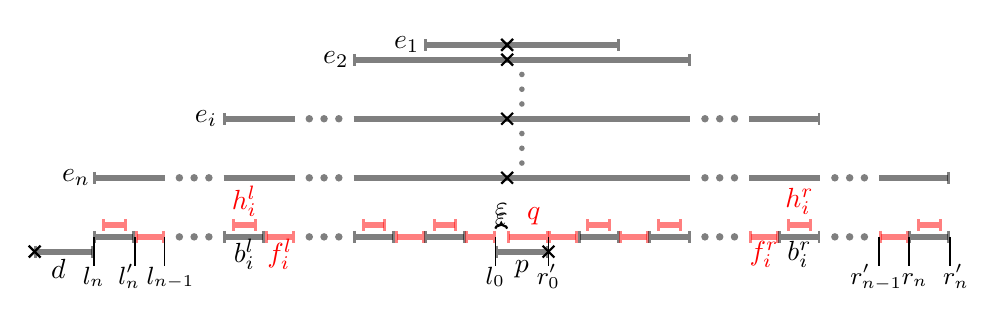
\begin{tikzpicture}[scale=0.75]
\definecolor{dgreen}{RGB}{0, 0, 0}
\usetikzlibrary{decorations.pathreplacing}
\draw[dgreen, opacity=0.5, line width=2.25pt]   (0.037500000000000006, 0) -- (0.9625, 0);
\draw[dgreen, opacity=0.5, line width=0.037500000000000006*1cm/1pt]      (0.018750000000000003, 0.1) -- (0.018750000000000003, -0.1);
\draw[dgreen, opacity=0.5, line width=0.037500000000000006*1cm/1pt]      (0.98125, 0.1) -- (0.98125, -0.1);
\node at (0.7, 1.25)  { $e_n$};
\draw[black, opacity=0.5, line width=2.25pt]   (1.0375, 1.25) -- (2.2, 1.25);
\draw[black, opacity=0.5, line width=0.037500000000000006*1cm/1pt]      (1.01875, 1.35) -- (1.01875, 1.15);
\node at (2.9000000000000004, 1.25)  { };
\draw[black, opacity=0.5, line width=2.25pt]   (3.2, 1.25) -- (4.4, 1.25);
\node at (2.9000000000000004, 2.25)  { $e_i$};
\draw[black, opacity=0.5, line width=2.25pt]   (3.2375000000000003, 2.25) -- (4.4, 2.25);
\draw[black, opacity=0.5, line width=0.037500000000000006*1cm/1pt]      (3.21875, 2.35) -- (3.21875, 2.15);
\node at (5.1000000000000005, 1.25)  { };
\draw[black, opacity=0.5, line width=2.25pt]   (5.4, 1.25) -- (11.099999999999998, 1.25);
\node at (5.1000000000000005, 2.25)  { };
\draw[black, opacity=0.5, line width=2.25pt]   (5.4, 2.25) -- (11.099999999999998, 2.25);
\node at (5.1000000000000005, 3.25)  { $e_2$};
\draw[black, opacity=0.5, line width=2.25pt]   (5.4375, 3.25) -- (11.062499999999998, 3.25);
\draw[black, opacity=0.5, line width=0.037500000000000006*1cm/1pt]      (5.41875, 3.35) -- (5.41875, 3.15);
\draw[black, opacity=0.5, line width=0.037500000000000006*1cm/1pt]      (11.081249999999997, 3.35) -- (11.081249999999997, 3.15);
\node at (6.300000000000001, 3.5)  { $e_1$};
\draw[black, opacity=0.5, line width=2.25pt]   (6.6375, 3.5) -- (9.862499999999999, 3.5);
\draw[black, opacity=0.5, line width=0.037500000000000006*1cm/1pt]      (6.61875, 3.6) -- (6.61875, 3.4);
\draw[black, opacity=0.5, line width=0.037500000000000006*1cm/1pt]      (9.881249999999998, 3.6) -- (9.881249999999998, 3.4);
\node at (11.799999999999997, 1.25)  { };
\draw[black, opacity=0.5, line width=2.25pt]   (12.099999999999998, 1.25) -- (13.299999999999997, 1.25);
\node at (11.799999999999997, 2.25)  { };
\draw[black, opacity=0.5, line width=2.25pt]   (12.099999999999998, 2.25) -- (13.262499999999998, 2.25);
\draw[black, opacity=0.5, line width=0.037500000000000006*1cm/1pt]      (13.281249999999996, 2.35) -- (13.281249999999996, 2.15);
\node at (13.999999999999996, 1.25)  { };
\draw[black, opacity=0.5, line width=2.25pt]   (14.299999999999997, 1.25) -- (15.462499999999997, 1.25);
\draw[black, opacity=0.5, line width=0.037500000000000006*1cm/1pt]      (15.481249999999996, 1.35) -- (15.481249999999996, 1.15);
\draw[dgreen, opacity=0.5, line width=2.25pt]   (1.0375, 0.25) -- (1.6624999999999999, 0.25);
\draw[dgreen, opacity=0.5, line width=0.037500000000000006*1cm/1pt]      (1.01875, 0.35) -- (1.01875, 0.15);
\draw[dgreen, opacity=0.5, line width=0.037500000000000006*1cm/1pt]      (1.68125, 0.35) -- (1.68125, 0.15);
\draw[red, opacity=0.5, line width=2.25pt]   (1.1875, 0.45) -- (1.5125, 0.45);
\draw[red, opacity=0.5, line width=0.037500000000000006*1cm/1pt]      (1.16875, 0.55) -- (1.16875, 0.35);
\draw[red, opacity=0.5, line width=0.037500000000000006*1cm/1pt]      (1.53125, 0.55) -- (1.53125, 0.35);
\draw[red, opacity=0.5, line width=2.25pt]   (1.7375, 0.25) -- (2.1625, 0.25);
\draw[red, opacity=0.5, line width=0.037500000000000006*1cm/1pt]      (1.71875, 0.35) -- (1.71875, 0.15);
\draw[red, opacity=0.5, line width=0.037500000000000006*1cm/1pt]      (2.1812500000000004, 0.35) -- (2.1812500000000004, 0.15);
\draw[dgreen, opacity=0.5, line width=2.25pt]   (3.2375000000000003, 0.25) -- (3.8625000000000003, 0.25);
\draw[dgreen, opacity=0.5, line width=0.037500000000000006*1cm/1pt]      (3.21875, 0.35) -- (3.21875, 0.15);
\draw[dgreen, opacity=0.5, line width=0.037500000000000006*1cm/1pt]      (3.8812500000000005, 0.35) -- (3.8812500000000005, 0.15);
\draw[red, opacity=0.5, line width=2.25pt]   (3.3875, 0.45) -- (3.7125000000000004, 0.45);
\draw[red, opacity=0.5, line width=0.037500000000000006*1cm/1pt]      (3.36875, 0.55) -- (3.36875, 0.35);
\draw[red, opacity=0.5, line width=0.037500000000000006*1cm/1pt]      (3.7312500000000006, 0.55) -- (3.7312500000000006, 0.35);
\draw[red, opacity=0.5, line width=2.25pt]   (3.9375000000000004, 0.25) -- (4.362500000000001, 0.25);
\draw[red, opacity=0.5, line width=0.037500000000000006*1cm/1pt]      (3.91875, 0.35) -- (3.91875, 0.15);
\draw[red, opacity=0.5, line width=0.037500000000000006*1cm/1pt]      (4.3812500000000005, 0.35) -- (4.3812500000000005, 0.15);
\draw[dgreen, opacity=0.5, line width=2.25pt]   (5.4375, 0.25) -- (6.062500000000001, 0.25);
\draw[dgreen, opacity=0.5, line width=0.037500000000000006*1cm/1pt]      (5.41875, 0.35) -- (5.41875, 0.15);
\draw[dgreen, opacity=0.5, line width=0.037500000000000006*1cm/1pt]      (6.081250000000001, 0.35) -- (6.081250000000001, 0.15);
\draw[red, opacity=0.5, line width=2.25pt]   (5.5875, 0.45) -- (5.9125000000000005, 0.45);
\draw[red, opacity=0.5, line width=0.037500000000000006*1cm/1pt]      (5.5687500000000005, 0.55) -- (5.5687500000000005, 0.35);
\draw[red, opacity=0.5, line width=0.037500000000000006*1cm/1pt]      (5.93125, 0.55) -- (5.93125, 0.35);
\draw[red, opacity=0.5, line width=2.25pt]   (6.1375, 0.25) -- (6.562500000000001, 0.25);
\draw[red, opacity=0.5, line width=0.037500000000000006*1cm/1pt]      (6.11875, 0.35) -- (6.11875, 0.15);
\draw[red, opacity=0.5, line width=0.037500000000000006*1cm/1pt]      (6.581250000000001, 0.35) -- (6.581250000000001, 0.15);
\draw[dgreen, opacity=0.5, line width=2.25pt]   (6.6375, 0.25) -- (7.262500000000001, 0.25);
\draw[dgreen, opacity=0.5, line width=0.037500000000000006*1cm/1pt]      (6.61875, 0.35) -- (6.61875, 0.15);
\draw[dgreen, opacity=0.5, line width=0.037500000000000006*1cm/1pt]      (7.281250000000001, 0.35) -- (7.281250000000001, 0.15);
\draw[red, opacity=0.5, line width=2.25pt]   (6.7875000000000005, 0.45) -- (7.112500000000001, 0.45);
\draw[red, opacity=0.5, line width=0.037500000000000006*1cm/1pt]      (6.768750000000001, 0.55) -- (6.768750000000001, 0.35);
\draw[red, opacity=0.5, line width=0.037500000000000006*1cm/1pt]      (7.1312500000000005, 0.55) -- (7.1312500000000005, 0.35);
\draw[red, opacity=0.5, line width=2.25pt]   (7.3375, 0.25) -- (7.762500000000001, 0.25);
\draw[red, opacity=0.5, line width=0.037500000000000006*1cm/1pt]      (7.3187500000000005, 0.35) -- (7.3187500000000005, 0.15);
\draw[red, opacity=0.5, line width=0.037500000000000006*1cm/1pt]      (7.781250000000001, 0.35) -- (7.781250000000001, 0.15);
\draw[dgreen, opacity=0.5, line width=2.25pt]   (7.8375, 0) -- (8.6625, 0);
\draw[dgreen, opacity=0.5, line width=0.037500000000000006*1cm/1pt]      (7.8187500000000005, 0.1) -- (7.8187500000000005, -0.1);
\draw[dgreen, opacity=0.5, line width=0.037500000000000006*1cm/1pt]      (8.681249999999999, 0.1) -- (8.681249999999999, -0.1);
\draw[red, opacity=0.5, line width=2.25pt]   (8.0375, 0.25) -- (8.6625, 0.25);
\draw[red, opacity=0.5, line width=0.037500000000000006*1cm/1pt]      (8.01875, 0.35) -- (8.01875, 0.15);
\draw[red, opacity=0.5, line width=0.037500000000000006*1cm/1pt]      (8.681249999999999, 0.35) -- (8.681249999999999, 0.15);
\draw[red, opacity=0.5, line width=2.25pt]   (8.737499999999999, 0.25) -- (9.1625, 0.25);
\draw[red, opacity=0.5, line width=0.037500000000000006*1cm/1pt]      (8.71875, 0.35) -- (8.71875, 0.15);
\draw[red, opacity=0.5, line width=0.037500000000000006*1cm/1pt]      (9.181249999999999, 0.35) -- (9.181249999999999, 0.15);
\draw[dgreen, opacity=0.5, line width=2.25pt]   (9.237499999999999, 0.25) -- (9.862499999999999, 0.25);
\draw[dgreen, opacity=0.5, line width=0.037500000000000006*1cm/1pt]      (9.21875, 0.35) -- (9.21875, 0.15);
\draw[dgreen, opacity=0.5, line width=0.037500000000000006*1cm/1pt]      (9.881249999999998, 0.35) -- (9.881249999999998, 0.15);
\draw[red, opacity=0.5, line width=2.25pt]   (9.3875, 0.45) -- (9.712499999999999, 0.45);
\draw[red, opacity=0.5, line width=0.037500000000000006*1cm/1pt]      (9.36875, 0.55) -- (9.36875, 0.35);
\draw[red, opacity=0.5, line width=0.037500000000000006*1cm/1pt]      (9.731249999999998, 0.55) -- (9.731249999999998, 0.35);
\draw[red, opacity=0.5, line width=2.25pt]   (9.937499999999998, 0.25) -- (10.362499999999999, 0.25);
\draw[red, opacity=0.5, line width=0.037500000000000006*1cm/1pt]      (9.91875, 0.35) -- (9.91875, 0.15);
\draw[red, opacity=0.5, line width=0.037500000000000006*1cm/1pt]      (10.381249999999998, 0.35) -- (10.381249999999998, 0.15);
\draw[dgreen, opacity=0.5, line width=2.25pt]   (10.437499999999998, 0.25) -- (11.062499999999998, 0.25);
\draw[dgreen, opacity=0.5, line width=0.037500000000000006*1cm/1pt]      (10.41875, 0.35) -- (10.41875, 0.15);
\draw[dgreen, opacity=0.5, line width=0.037500000000000006*1cm/1pt]      (11.081249999999997, 0.35) -- (11.081249999999997, 0.15);
\draw[red, opacity=0.5, line width=2.25pt]   (10.587499999999999, 0.45) -- (10.912499999999998, 0.45);
\draw[red, opacity=0.5, line width=0.037500000000000006*1cm/1pt]      (10.56875, 0.55) -- (10.56875, 0.35);
\draw[red, opacity=0.5, line width=0.037500000000000006*1cm/1pt]      (10.931249999999997, 0.55) -- (10.931249999999997, 0.35);
\draw[red, opacity=0.5, line width=2.25pt]   (12.137499999999998, 0.25) -- (12.562499999999998, 0.25);
\draw[red, opacity=0.5, line width=0.037500000000000006*1cm/1pt]      (12.118749999999999, 0.35) -- (12.118749999999999, 0.15);
\draw[red, opacity=0.5, line width=0.037500000000000006*1cm/1pt]      (12.581249999999997, 0.35) -- (12.581249999999997, 0.15);
\draw[dgreen, opacity=0.5, line width=2.25pt]   (12.637499999999998, 0.25) -- (13.262499999999998, 0.25);
\draw[dgreen, opacity=0.5, line width=0.037500000000000006*1cm/1pt]      (12.618749999999999, 0.35) -- (12.618749999999999, 0.15);
\draw[dgreen, opacity=0.5, line width=0.037500000000000006*1cm/1pt]      (13.281249999999996, 0.35) -- (13.281249999999996, 0.15);
\draw[red, opacity=0.5, line width=2.25pt]   (12.787499999999998, 0.45) -- (13.112499999999997, 0.45);
\draw[red, opacity=0.5, line width=0.037500000000000006*1cm/1pt]      (12.768749999999999, 0.55) -- (12.768749999999999, 0.35);
\draw[red, opacity=0.5, line width=0.037500000000000006*1cm/1pt]      (13.131249999999996, 0.55) -- (13.131249999999996, 0.35);
\draw[red, opacity=0.5, line width=2.25pt]   (14.337499999999997, 0.25) -- (14.762499999999998, 0.25);
\draw[red, opacity=0.5, line width=0.037500000000000006*1cm/1pt]      (14.318749999999998, 0.35) -- (14.318749999999998, 0.15);
\draw[red, opacity=0.5, line width=0.037500000000000006*1cm/1pt]      (14.781249999999996, 0.35) -- (14.781249999999996, 0.15);
\draw[dgreen, opacity=0.5, line width=2.25pt]   (14.837499999999997, 0.25) -- (15.462499999999997, 0.25);
\draw[dgreen, opacity=0.5, line width=0.037500000000000006*1cm/1pt]      (14.818749999999998, 0.35) -- (14.818749999999998, 0.15);
\draw[dgreen, opacity=0.5, line width=0.037500000000000006*1cm/1pt]      (15.481249999999996, 0.35) -- (15.481249999999996, 0.15);
\draw[red, opacity=0.5, line width=2.25pt]   (14.987499999999997, 0.45) -- (15.312499999999996, 0.45);
\draw[red, opacity=0.5, line width=0.037500000000000006*1cm/1pt]      (14.968749999999998, 0.55) -- (14.968749999999998, 0.35);
\draw[red, opacity=0.5, line width=0.037500000000000006*1cm/1pt]      (15.331249999999995, 0.55) -- (15.331249999999995, 0.35);
\draw[thick, decorate, decoration={brace, amplitude=2pt}] (7.800000000000001, 0.39) -- (8.0, 0.39) node[midway,yshift=7pt] {$\varepsilon$};
\draw[thick] (-0.1, -0.1) -- (0.1, 0.1);
\draw[thick] (0.1, -0.1) -- (-0.1, 0.1);
\draw[thick] (7.9, 1.15) -- (8.1, 1.35);
\draw[thick] (8.1, 1.15) -- (7.9, 1.35);
\draw[thick] (7.9, 2.15) -- (8.1, 2.35);
\draw[thick] (8.1, 2.15) -- (7.9, 2.35);
\draw[thick] (7.9, 3.15) -- (8.1, 3.35);
\draw[thick] (8.1, 3.15) -- (7.9, 3.35);
\draw[thick] (7.9, 3.4) -- (8.1, 3.6);
\draw[thick] (8.1, 3.4) -- (7.9, 3.6);
\draw[thick] (8.6, -0.1) -- (8.799999999999999, 0.1);
\draw[thick] (8.799999999999999, -0.1) -- (8.6, 0.1);
\node[] at (3.5500000000000003, -0.04999999999999999) {\color{dgreen}$b_i^l$};
\node[] at (3.5500000000000003, 0.85) {\color{red}$h_i^l$};
\node[] at (4.15, -0.04999999999999999) {\color{red}$f_i^l$};
\node[] at (12.949999999999998, 0.85) {\color{red}$h_i^r$};
\node[] at (12.949999999999998, -0.04999999999999999) {\color{dgreen}$b_i^r$};
\node[] at (12.349999999999998, -0.04999999999999999) {\color{red}$f_i^r$};
\node[] at (0.4, -0.3) {\color{dgreen}$d$};
\node[] at (8.25, -0.3) {\color{dgreen}$p$};
\node[] at (8.45, 0.6) {\color{red}$q$};
\node[] at (7.9, 0.55) {\color{black}$\varepsilon$};
\draw[black, line width=0.02*1cm/1pt] (1, 0.25) -- (1, -0.25);
\node[anchor=base] at (1, -0.55) {\small\color{black}$l_n$};
\draw[black, line width=0.02*1cm/1pt] (1.7, 0.25) -- (1.7, -0.25);
\node[anchor=base] at (1.5999999999999999, -0.55) {\small\color{black}$l_n'$};
\draw[black, line width=0.02*1cm/1pt] (14.799999999999997, 0.25) -- (14.799999999999997, -0.25);
\node[anchor=base] at (14.899999999999997, -0.55) {\small\color{black}$r_n$};
\draw[black, line width=0.02*1cm/1pt] (15.499999999999996, 0.25) -- (15.499999999999996, -0.25);
\node[anchor=base] at (15.599999999999996, -0.55) {\small\color{black}$r_n'$};
\draw[black, line width=0.02*1cm/1pt] (7.800000000000001, 0.25) -- (7.800000000000001, -0.25);
\node[anchor=base] at (7.800000000000001, -0.55) {\small\color{black}$l_0$};
\draw[black, line width=0.02*1cm/1pt] (8.7, 0.25) -- (8.7, -0.25);
\node[anchor=base] at (8.7, -0.55) {\small\color{black}$r_0'$};
\draw[black, line width=0.02*1cm/1pt] (2.2, 0.25) -- (2.2, -0.25);
\node[anchor=base] at (2.3000000000000003, -0.55) {\small\color{black}$l_{n-1}$};
\draw[black, line width=0.02*1cm/1pt] (14.299999999999997, 0.25) -- (14.299999999999997, -0.25);
\node[anchor=base] at (14.249999999999996, -0.55) {\small\color{black}$r_{n-1}'$};
\fill[opacity=0.5] (2.45, 0.25) circle (1.8pt);
\fill[opacity=0.5] (2.7, 0.25) circle (1.8pt);
\fill[opacity=0.5] (2.95, 0.25) circle (1.8pt);
\fill[opacity=0.5] (2.45, 1.25) circle (1.8pt);
\fill[opacity=0.5] (2.7, 1.25) circle (1.8pt);
\fill[opacity=0.5] (2.95, 1.25) circle (1.8pt);
\fill[opacity=0.5] (4.65, 0.25) circle (1.8pt);
\fill[opacity=0.5] (4.9, 0.25) circle (1.8pt);
\fill[opacity=0.5] (5.15, 0.25) circle (1.8pt);
\fill[opacity=0.5] (4.65, 1.25) circle (1.8pt);
\fill[opacity=0.5] (4.9, 1.25) circle (1.8pt);
\fill[opacity=0.5] (5.15, 1.25) circle (1.8pt);
\fill[opacity=0.5] (4.65, 2.25) circle (1.8pt);
\fill[opacity=0.5] (4.9, 2.25) circle (1.8pt);
\fill[opacity=0.5] (5.15, 2.25) circle (1.8pt);
\fill[opacity=0.5] (11.349999999999998, 0.25) circle (1.8pt);
\fill[opacity=0.5] (11.599999999999998, 0.25) circle (1.8pt);
\fill[opacity=0.5] (11.849999999999998, 0.25) circle (1.8pt);
\fill[opacity=0.5] (11.349999999999998, 1.25) circle (1.8pt);
\fill[opacity=0.5] (11.599999999999998, 1.25) circle (1.8pt);
\fill[opacity=0.5] (11.849999999999998, 1.25) circle (1.8pt);
\fill[opacity=0.5] (11.349999999999998, 2.25) circle (1.8pt);
\fill[opacity=0.5] (11.599999999999998, 2.25) circle (1.8pt);
\fill[opacity=0.5] (11.849999999999998, 2.25) circle (1.8pt);
\fill[opacity=0.5] (13.549999999999997, 0.25) circle (1.8pt);
\fill[opacity=0.5] (13.799999999999997, 0.25) circle (1.8pt);
\fill[opacity=0.5] (14.049999999999997, 0.25) circle (1.8pt);
\fill[opacity=0.5] (13.549999999999997, 1.25) circle (1.8pt);
\fill[opacity=0.5] (13.799999999999997, 1.25) circle (1.8pt);
\fill[opacity=0.5] (14.049999999999997, 1.25) circle (1.8pt);
\fill[opacity=0.5] (8.25, 1.5) circle (1.3499999999999999pt);
\fill[opacity=0.5] (8.25, 1.75) circle (1.3499999999999999pt);
\fill[opacity=0.5] (8.25, 2.0) circle (1.3499999999999999pt);
\fill[opacity=0.5] (8.25, 2.5) circle (1.3499999999999999pt);
\fill[opacity=0.5] (8.25, 2.75) circle (1.3499999999999999pt);
\fill[opacity=0.5] (8.25, 3.0) circle (1.3499999999999999pt);
\end{tikzpicture}%[Finished in 42ms]
    \caption{A sketch of the DDT-Line instance construction. There are $3n+2$ slow agents $\{e_i, b^l_i, b^r_i\}_{i\in [n]} \cup \{d, p\}$, $4n+1$ fast agents $\{f^l_i,f^r_i, h^l_i, h^r_i\}_{i\in [n]} \cup \{q\}$. The starting point $s$ is the leftmost node of agent $d$'s interval, and the destination $y$ is the rightmost point of agent $e_n$'s interval. In the middle part we have a gap of size $\varepsilon$ which can only be traversed by the $e_i$'s or $p$. Assigning $e_i$'s to the left side such that the respective $p_i$'s sum up to exactly $\frac{P}{2}$, the package meets $p$ at $l_0$ without waiting time.}
\label{fig:line_2speed}
\end{figure} 


Observe that in the DDT-Line instance, we have alternating slow ($b_i$) and fast ($f_i$) base agents covering the main part of the $s-y$ interval. These agents cover the entire range except for a small gap of length  $\varepsilon$ in the middle, which is covered by the designated package carrier $p$ as well as the element agents. However, the instance is designed in a way such that we will have to choose $p$ here to achieve optimal delivery time. The $f_i$ agents are strategically designed so that no optimal schedule can bypass them. For the intervals corresponding to $b_i$, we have two options: either stick entirely with $b_i$ or use $h_i$ and a feasible $e_i$. The idea is that agent $h_i$ only benefits our schedule if we deliver the package to it and then pick it up from its right-most point by ``another agent''; otherwise, simply staying with $b_i $ yields the same solution. This introduces the role of $e_i$ as the ``another agent''. An agent $e_i$ acts as the counterpart to $b_i$ by either delivering to or picking up from $h_i$'s interval. Although any $e_j$ with $j>i$ could also play the respective counterpart or even stand in for $b_i$, this will not happen for any optimal solution, as we will discuss later. A detailed illustration of the $b_i$ and $h_i$ construction is provided in Figure  \ref{fig:line_2speed_gadget}.  

\begin{figure}[ht]
    \centering
    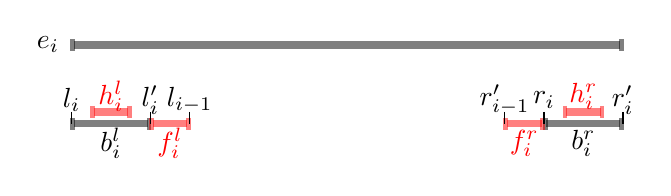
\begin{tikzpicture}[scale=0.5]
\definecolor{dgreen}{RGB}{13, 138, 8}
\draw[black, opacity=0.5, line width=2.7pt]   (11.06, 2) -- (24.94, 2);
\draw[black, opacity=0.5, line width=0.06*1cm/1pt]   (11.03, 2.15) -- (11.03, 1.85);
\draw[black, opacity=0.5, line width=0.06*1cm/1pt]   (24.97, 2.15) -- (24.97, 1.85);
\draw[black, opacity=0.5, line width=2.7pt]   (11.06, 0) -- (12.94, 0);
\draw[black, opacity=0.5, line width=0.06*1cm/1pt]   (11.03, 0.15) -- (11.03, -0.15);
\draw[black, opacity=0.5, line width=0.06*1cm/1pt]   (12.97, 0.15) -- (12.97, -0.15);
\draw[red, opacity=0.5, line width=2.7pt]   (11.56, 0.3) -- (12.44, 0.3);
\draw[red, opacity=0.5, line width=0.06*1cm/1pt]   (11.53, 0.44999999999999996) -- (11.53, 0.15);
\draw[red, opacity=0.5, line width=0.06*1cm/1pt]   (12.47, 0.44999999999999996) -- (12.47, 0.15);
\draw[red, opacity=0.5, line width=2.7pt]   (13.06, 0) -- (13.94, 0);
\draw[red, opacity=0.5, line width=0.06*1cm/1pt]   (13.03, 0.15) -- (13.03, -0.15);
\draw[red, opacity=0.5, line width=0.06*1cm/1pt]   (13.97, 0.15) -- (13.97, -0.15);
\draw[black, opacity=0.5, line width=2.7pt]   (23.06, 0) -- (24.94, 0);
\draw[black, opacity=0.5, line width=0.06*1cm/1pt]   (23.03, 0.15) -- (23.03, -0.15);
\draw[black, opacity=0.5, line width=0.06*1cm/1pt]   (24.97, 0.15) -- (24.97, -0.15);
\draw[red, opacity=0.5, line width=2.7pt]   (23.56, 0.3) -- (24.44, 0.3);
\draw[red, opacity=0.5, line width=0.06*1cm/1pt]   (23.53, 0.44999999999999996) -- (23.53, 0.15);
\draw[red, opacity=0.5, line width=0.06*1cm/1pt]   (24.47, 0.44999999999999996) -- (24.47, 0.15);
\draw[red, opacity=0.5, line width=2.7pt]   (22.06, 0) -- (22.94, 0);
\draw[red, opacity=0.5, line width=0.06*1cm/1pt]   (22.03, 0.15) -- (22.03, -0.15);
\draw[red, opacity=0.5, line width=0.06*1cm/1pt]   (22.97, 0.15) -- (22.97, -0.15);
\draw[black, line width=0.02*1cm/1pt]   (11, 0.3) -- (11, 0);
\draw[black, line width=0.02*1cm/1pt]   (13, 0.3) -- (13, 0);
\draw[black, line width=0.02*1cm/1pt]   (23, 0.3) -- (23, 0);
\draw[black, line width=0.02*1cm/1pt]   (25, 0.3) -- (25, 0);
\draw[black, line width=0.02*1cm/1pt]   (22, 0.3) -- (22, 0);
\draw[black, line width=0.02*1cm/1pt]   (14, 0.3) -- (14, 0);
\node[] at (12, -0.5) {\color{black}$b_i^l$};
\node[] at (13.5, -0.5) {\color{red}$f_i^l$};
\node[] at (24, -0.5) {\color{black}$b_i^r$};
\node[] at (22.5, -0.5) {\color{red}$f_i^r$};
\node[] at (10.4, 2) {\color{black}$e_i$};
\node[] at (12, 0.7) {\color{red}$h_i^l$};
\node[] at (24, 0.7) {\color{red}$h_i^r$};
\node[] at (14, 0.6) {\color{black}$l_{i-1}$};
\node[] at (11, 0.6) {\color{black}$l_i$};
\node[] at (13, 0.6) {\color{black}$l_i'$};
\node[] at (23, 0.6) {\color{black}$r_i$};
\node[] at (22, 0.6) {\color{black}$r_{i-1}'$};
\node[] at (25, 0.6) {\color{black}$r_i'$};
\end{tikzpicture}
    \caption{A close-up on $p_i$'s corresponding agents: slow agent $e_i$, $b_i^l $ and $ b_i^r$;  fast agents $f_i^l $, $ f_i^r$, $h_i^l$, and $ h_i^r$. From the construction, it is clear that  $e_i$ can only help only on either the left or right side interval, utilizing the fast drones $h_i$ on that side. A helping agent $h_i$ is utilized by assigning $e_i$ to either pick up the package from or deliver it to $h_i$. Not assigning $e_i$ leaves $h_i$ ineffective, as the delivery time is only dependent on $b_i$ as it has to catch up and pick up the package again.}
\label{fig:line_2speed_gadget}
\end{figure}


Building on the above observation, we will briefly outline the design goals for these intervals. 
It is important to note that the interval length of each agent $b_i$ depends on the underlying $p_i$, allowing us to construct both sides of the partition instance effectively. This means that the interval length of $b_i$ grows with the size $p_i$.  On the boundaries of the instance, the $b_i$'s have the largest lengths while they decrease as we move to the middle. It is clear that it benefits the delivery time the most if an element agent helps a larger $b_i$. To prevent any $e_i$ from helping any $b_j$ with $j>i$, we previously ordered the $p_i$ (and correspondingly the $e_i$) in increasing sequence and ensure that all $b_j$ with $j>i$ are inaccessible to $e_i$ (see Figure~\ref{fig:line_2speed}). As a result, $e_i$ can only help $b_j$ with $j\leq i$, while the optimal helping spot is then $b_i$ (either $b^l_i$ or  $b^r_i$). If $e_i$ would help at some $b_j$ with $j<i$ the schedule could be improved through an exchange argument. As large parts of the instance can be traversed with fast speed ($f_i$'s), it will not happen for any $e_i$ to help multiple $b_j$'s. This is exactly why there has to be made a choice between left and right by every $e_i$ to help a designated $b_j$ ($j\leq i$) which is $b_i^r$ or $b_i^l$ optimally.


To determine if the Partition instance is a ``yes''-instance, we use agent $p$. This agent is strategically positioned so that the package reaches agent $p$'s leftmost border precisely when the underlying $p_i$'s of the helping $e_i$'s sum up to exactly $\frac{P}{2}$ on the left side. Agent $p$ is positioned at its right border and upon initiating the delivery it starts moving to the left. Therefore we have to choose the length of $p$ to coincide with the exact time required to traverse the left side of the instance (including $d$) assuming we assign the $e_i$ agents corresponding to a feasible partition.
Only $p$ and all $e_i$ agents can traverse the middle part of our instance. The idea is that if we can not meet agent $p$ at the perfect time or use some agent $e_i$ instead of agent $p$ to traverse the middle gap, optimal delivery time cannot be achieved. %To make sure that $p$ does not help any $b_i^r$ (picking from or delivering the package to $h_i^r$), $p$ is (almost) completely covered by a fast agent $q$ which is supposed to travel over that middle part.   
Note that $p$ also cannot help any other $b_i^l$ or $b_i^r$ agents as there is no overlap between them.
There is another nuance to consider when it comes to the interval lengths of the agents $\{b^l_i\}_{i\in [n]}$. Assume for a moment that $b_i^l$ and $b_i^r$
were of equal length, we could achieve an optimal schedule without accurate partitioning – simply by assigning all agents to the right side, gaining the same benefits from helping and meeting $p$ on its left border after it has waited for the package. This strategy would result in the delivery time as if we had implemented a correct partition on both sides. To address this issue, we make  $b_i^l$ slightly larger by a factor of  $1+\frac{1}{P}$ to incentivize helping $b^l_i$. %Then it is clear, that we lose optimal delivery time by not considering the left side in the assignment as slower agents cover larger intervals.
Then it is clear, that we lose optimal delivery time by assigning more agents to the right side as slower agents cover larger intervals. On the other hand, assigning agents corresponding to more than $\frac{P}{2}$ to the right side results in the package having to wait for $p$ and thus also losing the optimal delivery time, therefore the optimal schedule assigns the agents corresponding to a feasible partition, if possible. For completeness, we now state a formal proof of Theorem \ref{thm:line} and give the precise construction.

\paragraph*{Proof of Theorem 1.}
\label{sec:appendixDDTL}
First, we formally define the instance, beginning with variables corresponding to the leftmost and rightmost points of the intervals: $l_i $ and $ l_i'$ for the left side of agent $p$'s interval, $r_i$ and $r_i'$ for right of agent $p$'s interval, respectively (see Figure \ref{fig:line_2speed} and \ref{fig:line_2speed_gadget}). For $l_n$, we define it as $l_n=(2n+2)P^2-\frac{P}{2}-\frac{n}{2}-\frac{1}{2P}-1 + \varepsilon$, which represents the length of delay agent $d$ (i.e.\ the offset from $0$). We can write the following recursions for the left side:
\begin{align*}
    \forall i\in\{1,...,n\}:\, l_i'=l_i+(1+\frac{1}{P})p_i \\
    \forall i\in\{0,...,n-1\}:\, l_i=l_{i+1}'+P
\end{align*}
Correspondingly for the right side we can write a similar recursion. Serving as the base, $r_0'=l_0+(2n+2)P^2+\varepsilon$. It follows that
\begin{align*}
    \forall i\in\{1,...,n\}: r_i'=r_i+p_i \\
    \forall i\in\{1,...,n\}: r_i=r_{i-1}'+P.
\end{align*}
We can now define all agents' movement intervals using the above specified variables. Figure \ref{fig:line_2speed} also illustrates the structure of these variables. The available speeds are $1$ and $2P$. We define agent set $A$  to include: 
\begin{itemize}
    \item[$\bullet$] $d=(0,1,[0,l_n])$
    \item[$\bullet$] $p$ = $(r_0',1,[l_0,r_0'])$ 
    \item[$\bullet$] $q$ = $(r_0',2P,[l_0+\varepsilon,r_0'])$
    \item[$\bullet$] $\forall i\{1,...,n\}: b_i^l=(l_i,1,[l_i,l_i'])$
    \item[$\bullet$] $\forall i\{1,...,n\}: f_i^l=(l_i',2P,[l_i',l_{i-1}])$
    \item[$\bullet$] $\forall i\{1,...,n\}: b_i^r=(r_i,1,[r_i,r_i'])$
    \item[$\bullet$] $\forall i\{1,...,n\}: f_i^r=(r_{i-1}',2P,[r_{i-1}',r_i])$
    \item[$\bullet$] $\forall i\{1,...,n\}: e_i = (l_0+\varepsilon,1,[l_i,r_i'])$
    \item[$\bullet$] $\forall i\{1,...,n\}: h_i^l=(l_i+\delta,2P,[l_i+\delta,l_i'-\delta])$ with $\delta=(1+\frac{1}{P})\frac{p_i}{4P-2}$
    \item[$\bullet$] $\forall i\{1,...,n\}: h_i^r=(r_i+\delta',2P,[r_i+\delta',r_i'-\delta']$ with $\delta'=\frac{p_i}{4P-2}$
\end{itemize}

The value $\delta$ ($\delta'$ resp.) is chosen in a way such that the delivery time over the interval corresponding to $b_i^l$ ($b_i^r$) is $(1+\frac{1}{P})p_i$ ($p_i$) if there is no help and $(1+\frac{1}{P})\frac{p_i}{P}$ ($\frac{p_i}{P})$ otherwise. Essentially, a factor of $\frac{1}{P}$ is saved over the interval $b_i$ by assigning a suitable $e_j$ to help – optimally $e_i$ for the fastest overall schedule.

Consider the package to be $(0,r_n')$. 
We want to prove that the input of Partition is a ``yes''-instance if and only if there exists a schedule of time at most $t=(2n+2)P^2+(n+\frac{3}{2})P + \frac{n}{2} + \frac{1}{2} + 2\varepsilon$. Note that this is exactly the time a schedule needs if a feasible solution for Partition is assigned to each side of the DDT-Line instance. The threshold time $t$ exactly captures our previous observations: We assign element agents $e_i$ to both sides such that their underlying $p_i$'s sum up to exactly $\frac{P}{2}$; therefore we meet $p$ exactly on arrival at $l_0$ carrying the package over the gap and from there utilizing $q$ and proceeding with the right part of the instance.
 
On the other hand, if the underlying Partition instance is a ``no''-instance, then we can not beat the threshold time $t$. We argue that it is not feasible to skip agent $p$ or any $\{f_i^l, f_i^r\}_{i\in [n]}$. Assuming this is true, if we do not meet $p$ at the perfect time, the package either has to wait for agent $p$, or agent $p$ has to wait for the package.
In either case, achieving the desired threshold time is unattainable. In the first case, agents on the right cannot make up for the delay, and in the second case, we lost too much time on the left side as the intervals (corresponding to the $b_i^l$) are slightly larger. 

% \begin{proof}
%     We want to prove that the input of Partition is a ``yes''-instance if and only if there exists a schedule of time at most $t=(2n+2)P^2+(n+\frac{3}{2})P + \frac{1}{2} + 2\varepsilon$. Note that this is exactly the time schedule needs assigning a correct solution for Partition to each side of the DDTL instance. Notice by the choice of the length of the helping agents ($h_i^l$ and $h_i^r$) that the time to traverse the interval corresponding to $b_i$ is equal to $p_i$ with no help ($b_i$ carries package entirely) and with help shrinks to $\frac{p_i}{P}$ ($h_i$ carries over its subpart, $e_i$ and $b_i$ do the rest).
    
We will show two different lemmas to help proving our statement.


    \begin{lemma}
    \label{lemma:noskip}
        Any optimal schedule does not skip any agent $f_i^l$ or $f_i^r$ for all $i\in \{1, \dots, n\}$.
    \end{lemma}
    \begin{proof}
        Assume we want to skip any of the $f_i^l$. The only reason might be that we want to use the corresponding $e_i$ to pick up the package from $h_i^l$ and delivers it to $h_{i-1}^l$. That means $e_i$ carries the package over an additional distance $P$ and we therefore can get value from two helping agents using only one element agent. We assume we are at the left side of the instance as it is more beneficial regarding the helping agents. For the right side the same steps can be repeated.

        Let us compare the delivery times: First of all we have the time of the skipping strategy which is $t_{skip}=(1+\frac{1}{P})(\frac{p_i+p_{i-1}}{P})+P$ for some $i\geq 2$. The delivery time whenever we do not skip $f_i^l$ and not get helped with any of the adjacent intervals is $t_f=(1+\frac{1}{P})(p_i + p_{i-1}) + \frac{1}{2}$.

        It holds that $t_f<t_{skip}$, since

        \begin{align*}
                   (1+\frac{1}{P})(p_i+p_{i-1})+\frac{1}{2} &< (1+\frac{1}{P})(\frac{p_i+p_{i-1}}{P})+P\\
                    p_i + p_{i-1} + \frac{1}{2} &< \frac{p_i+p_{i-1}}{P^2} + \sum_{j\in[n]}p_j\\
                    \frac{1}{2} &< \frac{p_i+p_{i-1}}{P^2} + \sum_{j\in[n]\setminus\{i-1,i\}}p_j,
        \end{align*}
        where the last term is always true for any $n\geq 3$ as every input integer for Partition is at least 1. 
    \end{proof}

    We continue by arguing that is not possible to skip agent $p$. 

    \begin{lemma}
        \label{lemma:skipp}
        A schedule skipping $p$ does not deliver the package within time $t$.
    \end{lemma}

    \begin{proof}
     If we want to skip agent $p$ we have to assign some element agent (say $e_1$ as it has the least impact) to carry the package over the gap. However, if we do not use $p$ anyway we might as well get all gains on the left side as they are more beneficial by a factor $1+\frac{1}{P}$. The resulting strategy (call it the \emph{greedy strategy}) is the fastest among those skipping $p$. Lemma \ref{lemma:noskip} implies that all $f_i$ are part of our solutions. Therefore the proposed strategy differs only in the assignment of the element agents. The delay, the $f_i$ agents, as well as the middle part (agent $q$ as well as $p$ or $e_1$) have to be present in all schedules.
     This boils down the differences in delivery time to $t_{greedy}= (1+\frac{1}{P})(\frac{\sum_{2}^n p_j}{P}+p_1)+P$ for the greedy strategy. The first term result from the greedy left part and the second part represents the right part. For the schedule utilizing a perfect partition we have that $t^*=(1+\frac{1}{P})(\frac{1}{2}+\frac{P}{2})+ \frac{1}{2}+\frac{P}{2}$, where once again the first term represents the left side  and the other terms represent the right side of the instance. We want to show that $t^*<t_{greedy}$. Observe that $t^*=P + \frac{3}{2} + \frac{1}{2P}$ and $t_{greedy}= P + p_1 + 1 + \frac{1}{P} - \frac{p_1}{P^2}$. Together we get that

     \begin{align*}
        \frac{1}{2} + \frac{1}{2P} < p_1 + \frac{1}{P} - \frac{p_1}{P^2},
     \end{align*}
     which is true since $p_1\geq 1$ and $\frac{p_1}{P^2} \leq \frac{1}{2}$ for $n\geq 2$, proving the lemma.      
    \end{proof}

    Lemma \ref{lemma:noskip} together with Lemma \ref{lemma:skipp} imply that a schedule beating time $t$ needs to use $p$ to carry the package over the gap and assign each element agent $e_i$ to exactly one base agent $b_i$. With the instance construction and lemmas established, we are now ready to prove the following. 

\thmline* 

\begin{proof}
    Assume the input $M$ of Partition is a ``no''-instance, that is, there exists no subset $S\subset M$ with $\sum_{i\in S} p_i = \frac{P}{2}$. This implies that we can not meet $p$ at the perfect time. Either we allocate too little to the left side or too much. In the first case $p$ has to wait at the gap for the package. The gain that is made on the right side is smaller (by a factor of $\frac{1}{P}$) than a perfect partition could have achieved on the left side. Therefore we are too slow in this case. On the other hand, allocating too much to the left results in the package having to wait for $p$ to arrive. Thus the left side is just as fast as if we put a perfect partition. Since a perfect partition has more capacities on the right side, also overshooting on the left side results in a schedule that is too slow.

    There is another nuance to mention. So far we did not show that every agent can reach its desired helping spot in time. This case is especially crucial for agent $e_n$ if it wants to help on the right side. Agent $e_n$, as all element agents, starts at $l_0+\varepsilon$ and has to travel over the stretch (agent $q$). We demonstrate that $e_n$ has enough time to reach $r_n$ (and also $l_n$).

Assume that the input for Partition is a ``yes''-instance. Observe that if $e_n$ starts moving to the right as soon as possible it will be at $r_0'+\varepsilon$ whenever $p$ picks up the package at $l_0$. To reach $r_n$ agent $e_n$ has to travel distance $P-p_n+nP$ taking an equal amount of time $t_{e_n}$. We proceed with a pessimistic analysis: Assume for every $b_i^r$ with $1\leq i<n$ that it is helped. Then the package needs time $t_{package}=\frac{(2n+2)P^2}{2P} +\frac{nP}{2P}+1- \frac{p_n}{P}$, where the first term represents the stretch (agent $q$), the second term all $f_i^r$ and the last two terms the helped base agents. It holds that $t_{e_n}<t_{package}$ since

\begin{align*}
    (n+1)P - p_n &< \frac{(2n+2)P^2}{2P} +\frac{nP}{2P}+1- \frac{p_n}{P}\\
    (n+1)P - p_n &<(n+1)P + \frac{n}{2} + 1 - \frac{p_n}{P}\\
    - p_n &< \frac{n}{2} + 1 - \frac{p_n}{P}
\end{align*}
is true. 

In a similar fashion we can state that $e_n$ has enough time to reach $l_n$, i.e.\ the helping spot on the left side. Starting from $l_0 +\varepsilon$ it takes agent $e_n$ time $nP+(1+\frac{1}{P})P+\varepsilon$ to reach $l_n$. Due to the delay the package arrives at $l_n$ at time $(2n+2)P^2-\frac{P}{2}-1-\frac{1}{2P} + \varepsilon$, which is a sufficient amount of time for $n\geq 2$. As a consequence, $e_n$ has enough time to reach $l_n$. Together with the previous analysis we argued that all agents have enough time to reach their helping spot.

All in all we argued that there can not exist a schedule beating time $t$ whenever the underlying Partition input does not admit a perfect partition. This concludes the proof of Theorem \ref{thm:line}.
\end{proof}
It is said that we presented only a set of feasible values. There exist many more feasible values for speeds and distances that serve our construction.
\section{Hardness result on a grid}
\label{npgrid}
%\todo{maybe we could add a small paragraph somewhere that unit speed rectangular movement area is easy to solve. Andi: i like the idea}
% 

In this section, we study the DDT problem on grid graphs. The grid graph serves as the natural intermediary between a line and a general graph, and they are more closely aligned with applications such as road networks.  Formally, we define a grid graph as follows: The set of vertices is a finite set of integer coordinates $V \subset \mathbb{Z}^2$. 
%For any point with coordinates $x$ and $y$ on the grid, there exists a set of vertices $\{ (a, b)| a,b\in \mathbb{N}, -x \leq a\leq x, -y \leq b\leq y\}$ on the grid. 
An edge of length $1$ connects any two vertices if and only if exactly one of their coordinates differs by exactly one. Therefore we also refer to our grid graph as a \emph{unit grid}. We denote the DDT problem on the unit grid as DDT-Grid. %\todo{simon: can be maybe change this to allow negative coordinates? Andi: i dont see the immediate use of negative coordinates,simon: i use them in my construction. OK, simon: 2 alternatives below}
%For given boundaries $[x_1, x_2]$ and $[y_1, y_2]$ we have the set of vertices $V = \mathbb{Z}^2 \cap [x_1, x_2] \times [y_1, y_2]$.
%For given boundaries $[x_1, x_2]$ and $[y_1, y_2]$ we have a vertex $(x, y) \in \mathbb{Z}^2$ with $x \in [x_1, x_2]$ and $y \in [y_1, y_2]$.




% We will study two cases of DDT problem on grid graphs: the first involves rectangular movement areas with two speeds, discussed in Section~\ref{2grid}, and the second involves arbitrary movement areas with unit speeds in Section~\ref{1grid}. 
% Detailed notations for both cases are provided in the subsequent sections, with Figure~\ref{fig:rectangular_example} offering illustrative examples for each. 

\begin{figure}[ht]
    \centering
    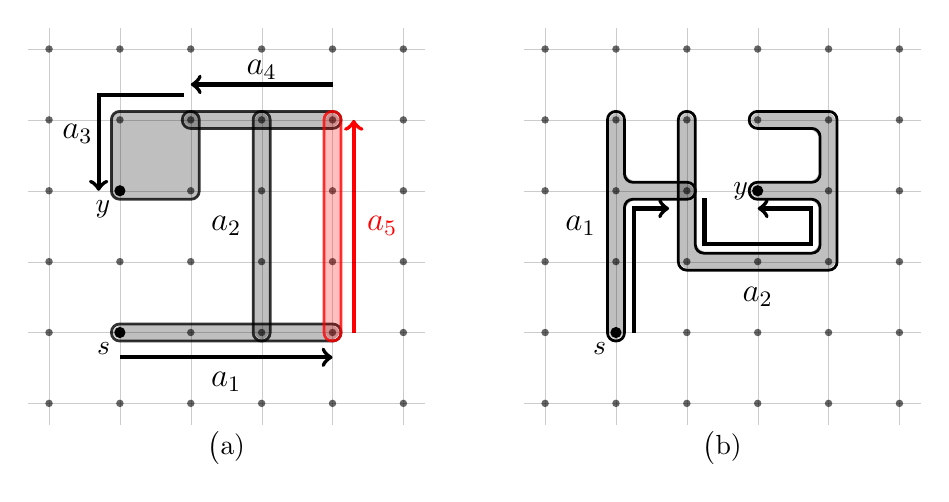
\begin{tikzpicture}[scale=0.9]
\definecolor{b1}{RGB}{0, 0, 0}
\definecolor{b2}{RGB}{4, 75, 145}
\definecolor{b3}{RGB}{76, 68, 194}
\definecolor{b4}{RGB}{50, 140, 190}
\draw[->, line width=1.5] (0, -0.35) -- (3, -0.35);
%\draw[->, dashed, red, line width=1.5] (3.35, 3) -- (3.35, 0);
\draw[<-, red, line width=1.5] (3.3, 3) -- (3.3, 0);
\draw[->, line width=1.5] (3, 3.5000000000000003) -- (1, 3.5000000000000003);
%\draw[<-, dashed, line width=1.5] (3, 3.45) -- (1.1, 3.45);
%\draw[->, dashed, line width=1.5] (1.35, 2) -- (1.35, 2.85);
\draw[->, line width=1.5] (0.9, 3.35) -- (-0.3, 3.35) -- (-0.3, 2);
\def\wi{0.08}
\def\op{0.2}
\def\pts{2.0pt}

\foreach \y in {-1, ...,4} {
\draw[black, line width=\wi, opacity=\op] (-1.3, \y) -- (4.3, \y);
\draw[black, line width=\wi, opacity=\op] (5.7, \y) -- (11.3, \y);
%\draw[black, line width=\wi, opacity=\op] (-46.3, \y) -- (-28.7, \y);
}
\foreach \x in {-1, 0, 1, 2, 3, 4, 6, 7, 8, 9, 10, 11} {
\draw[black, line width=\wi, opacity=\op] (\x, -1.3) -- (\x, 4.3);
%\draw[black, line width=\wi, opacity=\op] (\x, 5.7) -- (\x, 11.3);
%\draw[black, line width=\wi, opacity=\op] (-46.3, \y) -- (-28.7, \y);
}

% \foreach \y in {0,...,23} {
% \draw[black, line width=\wi, opacity=\op] (-25.3, \y) -- (3.3, \y);
% \draw[black, line width=\wi, opacity=\op] (-46.3, \y) -- (-28.7, \y);
% }

\foreach \x in {-1,...,4} {
\foreach \y in {-1,...,4} {
\fill[black, opacity=0.6] (\x, \y) circle (1.5pt);
}
}
\foreach \x in {6,...,11} {
\foreach \y in {-1,...,4} {
\fill[black, opacity=0.6] (\x, \y) circle (1.5pt);
}
}
\draw[b1, line width=1pt, opacity=0.8, rounded corners=3pt] (-0.12, -0.12) rectangle (3.12, 0.12);
\fill[b1, opacity=0.25, rounded corners=5pt] (-0.12, -0.12) rectangle (3.12, 0.12);

\draw[b1, line width=1pt, opacity=0.8, rounded corners=3pt] (1.88, -0.12) rectangle (2.12, 3.12);
\fill[b1, opacity=0.25, rounded corners=5pt] (1.88, -0.12) rectangle (2.12, 3.12);
\draw[b1, line width=1pt, opacity=0.8, rounded corners=3pt] (0.88, 2.88) rectangle (3.12, 3.12);
\fill[b1, opacity=0.25, rounded corners=5pt] (0.88, 2.88) rectangle (3.12, 3.12);
\draw[red, line width=1pt, opacity=0.8, rounded corners=3pt] (2.88, -0.12) rectangle (3.12, 3.12);
\fill[red, opacity=0.25, rounded corners=5pt] (2.88, -0.12) rectangle (3.12, 3.12);
\draw[b1, line width=1pt, opacity=0.8, rounded corners=3pt] (-0.12, 1.88) rectangle (1.12, 3.12);
\fill[b1, opacity=0.25, rounded corners=3pt] (-0.12, 1.88) rectangle (1.12, 3.12);
\draw[black, line width=1pt, rounded corners=3pt](7.88, 3.12) -- (7.88, 0.88) -- (10.120000000000001, 0.88) -- (10.120000000000001, 3.12) -- (8.88, 3.12) -- (8.88, 2.88) -- (9.879999999999999, 2.88) -- (9.879999999999999, 2.12) -- (8.88, 2.12) -- (8.88, 1.88) -- (9.879999999999999, 1.88) -- (9.879999999999999, 1.12) -- (8.12, 1.12) -- (8.12, 3.12) -- cycle;
\fill[black, opacity=0.25, rounded corners=5pt](7.88, 3.12) -- (7.88, 0.88) -- (10.120000000000001, 0.88) -- (10.120000000000001, 3.12) -- (8.88, 3.12) -- (8.88, 2.88) -- (9.879999999999999, 2.88) -- (9.879999999999999, 2.12) -- (8.88, 2.12) -- (8.88, 1.88) -- (9.879999999999999, 1.88) -- (9.879999999999999, 1.12) -- (8.12, 1.12) -- (8.12, 3.12) -- cycle;
\draw[black, line width=1pt, rounded corners=3pt](6.88, -0.12) -- (6.88, 3.12) -- (7.12, 3.12) -- (7.12, 2.12) -- (8.120000000000001, 2.12) -- (8.120000000000001, 1.88) -- (7.12, 1.88) -- (7.12, -0.12) -- cycle;
\fill[black, opacity=0.25, rounded corners=5pt](6.88, -0.12) -- (6.88, 3.12) -- (7.12, 3.12) -- (7.12, 2.12) -- (8.120000000000001, 2.12) -- (8.120000000000001, 1.88) -- (7.12, 1.88) -- (7.12, -0.12) -- cycle;
%\draw[->, dashed, line width=1.5] (6.75, 1) -- (6.75, 0);
\draw[->, line width=1.5] (7.25, 0) -- (7.25, 1.75) -- (7.75, 1.75);
\draw[->, line width=1.5] (8.25, 1.9) -- (8.25, 1.25) -- (9.75, 1.25) -- (9.75, 1.75) -- (9, 1.75);
%\draw[->, dashed, line width=1.5] (8.25, 3) -- (8.25, 2.1);
\filldraw (7, 0) circle (2pt);
\node[below left] at (7, 0) {$s$};
\filldraw (0, 2) circle (2pt);
\node[below left] at (0, 2) {$y$};
\filldraw (9, 2) circle (2pt);
\node[left] at (9, 2) {$y$};
\filldraw (0, 0) circle (2pt);
\node[below left] at (0, 0) {$s$};
% \filldraw[red] (3, 3) circle (2pt);
% \node[above right] at (3, 3) {\textcolor{red}{$p_5$}};
% \filldraw (2, 3) circle (2pt);
\node[] at (9, 0.5) {\large $a_2$};
\node[] at (1.5, 1.5) {\large $a_2$};
\node[] at (1.5, -0.7) {\large $a_1$};
\node[] at (6.5, 1.5) {\large $a_1$};
\node[red] at (3.7, 1.5) {\large $a_5$};
\node[] at (-0.6, 2.8) {\large $a_3$};
\node[] at (2, 3.7) {\large $a_4$};
% \filldraw (1, 2) circle (2pt);
% \node[below right] at (1, 2) {$p_3$};
% \filldraw (1, 3) circle (2pt);
% \node[above right] at (1, 3) {$p_4$};
% \filldraw (0, 3) circle (2pt);
% \node[above left] at (0, 3) {$y$};
% \filldraw (7, 1) circle (2pt);
% \node[above left] at (7, 1) {$p_1$};
% \filldraw (8, 3) circle (2pt);
%\node[above] at (8, 3) {$p_2$};
\node[above] at (1.5, -2) {\big (a)};
\node[above] at (8.5, -2) {\big (b)};
\end{tikzpicture}
%[Finished in 0.2s]
    \caption{Two DDT-Grid instances. On the left is an instance (a) where agents have rectangular movement areas and have two distinct speeds: %On the left, an instance (a) where agents have rectangular movement areas and two speeds:  
    %\simon{
    %  An example of a DDTGR instance with rectangular movement areas different speeds on the left and a DDTG instance with unit speed on the right: In the DDTGR instance, 
    there are four slow agents with speed $1$ and one fast agent with speed $5$, displayed black and red respectively. Each movement area is represented as a rectangle, indicated by shading. 
   % The movement areas represent a rectangle. 
   The optimal solution, with the respective trips indicated by bold solid arrows, takes a total time of $7.6$ by sequentially using agents $a_1 $, $ a_5$, $a_4$ and $ a_3$ to deliver the package from $s$ to $y$. %\andi{ The respective trips are indicated by the bold solid arrows. }
   On the right is an instance (b) with two agents having unit speed, where the movement areas of the agents are not rectangular.
    %On the right is an instance (b) where the movement areas of the agents are not rectangular and there are two agents with speed $1$.
    %On the right, an instance (b) where both movement areas of the drones are not rectangular.
   % In the DDTG instance on the right, 
    %there are two drones with speed $1$, distinguished in the figure by their start points $p_1$ and $p_2$ and their bounded movement subgraphs.  
    Note that even though the nodes of the subgraph of the second agent have rectangular shape, it is not a rectangular movement area as some edges are missing. The optimal solution takes a total time of $8$ by first using agent $a_1$ and then $a_2$ as indicated by the bold solid arrows.}
    \label{fig:rectangular_example}
\end{figure}

We will study the case of DDT-Grid involving agents that are restricted to rectangular movement areas. 
This restriction to rectangular movement areas is natural, reflecting real-world scenarios where agents' movements are typically constrained to specific, license-determined, convex areas, such as road networks.  
Let us define what constitutes a \emph{rectangular} movement area: For every agent $a$, the vertex set $V_a$ forms a rectangular shape, i.e., for every two vertices $x=(x_1,x_2) \in V_a$ and $y=(y_1,y_2)\in V_a$ with $x_1\leq y_1$ and $x_2\leq y_2$, every vertex $z=(z_1,z_2) \in \mathbb{Z}^2$ with $z_1 \in [x_1,y_1]$ and $z_2\in [x_2,y_2]$ must also belong to $V_a$. Regarding $E_a$, for every pair of vertices in $V_a$ differing by exactly 1 in one coordinate, the connecting edge $e$ must be in $E_a$. Intuitively, this ensures that the subgraph forms a rectangle where every possible vertex and edge within that rectangle is included.  This specific scenario will be referred to as DDT-GridR.  
An example of rectangular as well as arbitrary movement areas is given in Figure \ref{fig:rectangular_example}.  

If all agents have the same speed, we can easily provide a polynomial-time algorithm to solve the above DDT-GridR problem without initial positions by constructing the shortest path and generating the corresponding collaborative schedule. However, when agents operate at two different speeds, the problem becomes significantly more complex and challenging.  
We now state the main result regarding this setting. Notice that now unlike in section \ref{npline} we consider the setting of \emph{no initial positioning}. This means we have the flexibility to choose the initial placement of an agent rather than being constrained to fixed starting positions. We refer to the number of vertices $n$ in the grid graph as the \textit{size} of the grid.


\thmgrid*

% \textcolor{blue}{Note that our results from Theorem \ref{thm:line} directly transfer to the case of initial positions. As the movement areas on the line are considered rectangular, we can think of a grid where every agent is positioned on a single grid line. Adapting the construction yields the desired results in the case of fixed starting positions.}

% \andi{I dont think this is actually that easily transferred. The problem I see is that now we have unit grid (or at least equal distance between vertices) and also in the construction there might occur rational values (with the $\frac{1}{P}$ stuff). Maybe we just write that the general ideas could be adapted for the initial position setting if done carefully.}
% \simon{I agree I think it doesn't carry at all, as we use exponential values for the edges in our proof on the Line, which we can't do here as it requires exponential number of node; but maybe this is interesting to write why in our definitions DDT on a path is not a special case of DDT on a grid, because otherwise it may be confusing for reviewers}

 We prove the theorem by showing a reduction from \textsc{2P1N-3SAT}, a special case of \textsc{3SAT}, where each variable in the input formula appears exactly two times as a positive and one time as negative literal. 
 %, and each clause contains at most three literals.  
It is known, that \textsc{2P1N-3SAT} is NP-hard \cite{ryo:2p1nsat}. 
As in Section~\ref{npline}, we will provide a high-level overview of the construction first and later in this section give a formal proof.

%\andi{As previously in section~\ref{npgrid}, due to space limitations we will give a high level overview of the construction in this section. For the detailed construction as well as the complete proof please refer to Appendix~\ref{sec:appendixddtgrapx}.

Let $\phi$, with $n'$ variables and $m'$ clauses, be an instance of the \textsc{2P1N-3SAT} problem. 
The core idea behind the construction of the reduction instance is as follows: For every (of the three) occurrences of each variable we construct an agent which has to make a choice – help with solving the clauses (clause gadgets) or do not help (variable gadgets). Intuitively, the first refers to the literal being set to true, while the latter refers to the literal being set to false in the corresponding assignment.
%Intuitively, the first refers to the literal appearing as positive, while the latter refers to the literal appearing as negative.  
%the first refers to the literal being set to true whereas the latter refers to the literal being set to false.
The design goal of the variable gadgets is to ensure that every assignment is consistent, i.e.\ if $x_i$ is set to true then $\neg x_i$ is set to false. The idea of the clause gadgets is to make sure that the assignment fulfills every clause of the formula. We obtain that the optimal delivery time is below a certain threshold if and only if the given input $\phi$ of \textsc{2P1N-3SAT} is a ``yes''-instance. Furthermore, the DDT-GridR instance is constructed in a way, such that if $\phi$ is not satisfiable, then the additional delivery time increases drastically.


\begin{figure}[h!]
    \centering
    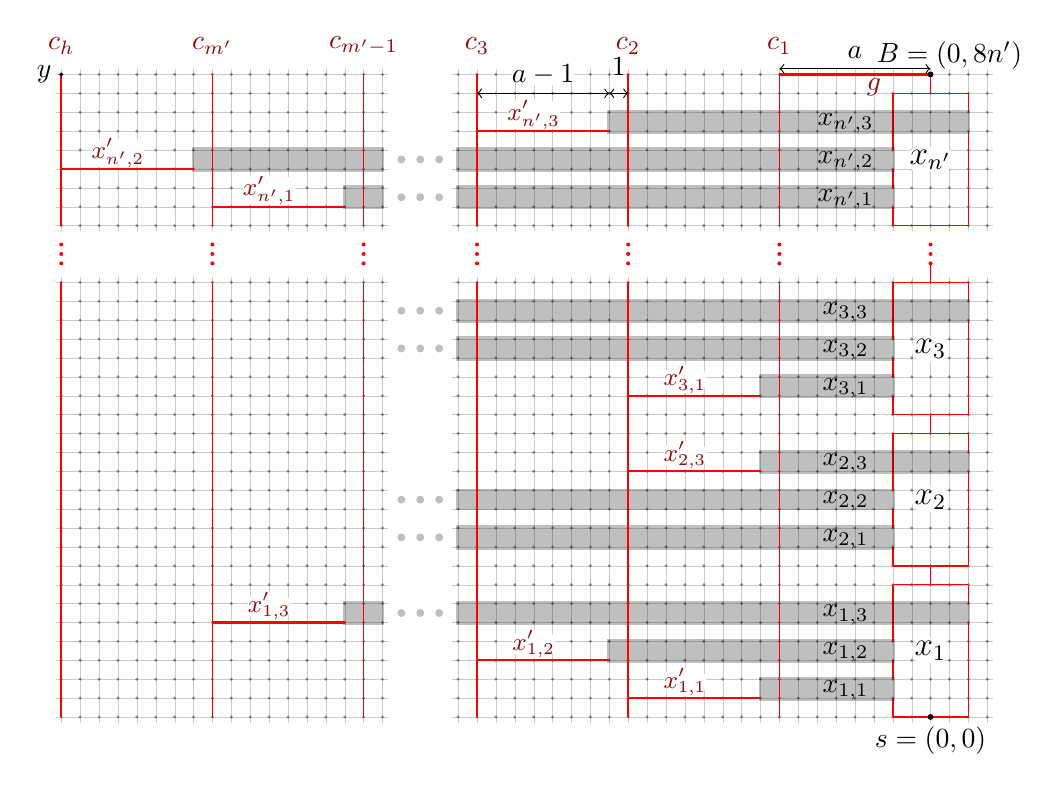
\begin{tikzpicture}[scale=0.24]
\definecolor{dred}{RGB}{143, 11, 11}
\def\wi{0.08}
\def\op{0.2}
\def\pts{2.5pt}

\foreach \x in {-25,...,3} {
\foreach \y in {0,...,23} {
\fill[black, opacity=0.4] (\x, \y) circle (\pts);
}
\draw[black, line width=\wi, opacity=\op] (\x, -0.3) -- (\x, 23.3);
}
\foreach \y in {0,...,23} {
\draw[black, line width=\wi, opacity=\op] (-25.3, \y) -- (3.3, \y);
\draw[black, line width=\wi, opacity=\op] (-46.3, \y) -- (-28.7, \y);
}
\foreach \y in {26,...,34} {
\draw[black, line width=\wi, opacity=\op] (-25.3, \y) -- (3.3, \y);
\draw[black, line width=\wi, opacity=\op] (-46.3, \y) -- (-28.7, \y);
}

\foreach \x in {-25,...,3} {
\foreach \y in {26,...,34} {
\fill[black, opacity=0.4] (\x, \y) circle (\pts);
}
\draw[black, line width=\wi, opacity=\op] (\x, 25.7) -- (\x, 34.3);
}


\foreach \x in {-46,...,-29} {
\foreach \y in {26,...,34} {
\fill[black, opacity=0.4] (\x, \y) circle (\pts);
}
\draw[black, line width=\wi, opacity=\op] (\x, 25.7) -- (\x, 34.3);

}
\foreach \x in {-46,...,-29} {
\foreach \y in {0,...,23} {
\fill[black, opacity=0.4] (\x, \y) circle (\pts);
}
\draw[black, line width=\wi, opacity=\op] (\x, -0.3) -- (\x, 23.3);
}
\draw[red, line width = 0.5669291340000001pt]   (-2, 0) -- (2, 0);
\draw[red, line width = 0.5669291340000001pt]   (-2, 0) -- (-2, 1);
\draw[red, line width = 0.5669291340000001pt]   (-2, 2) -- (-2, 3);
\draw[red, line width = 0.5669291340000001pt]   (-2, 4) -- (-2, 7);
\draw[red, line width = 0.5669291340000001pt]   (2, 0) -- (2, 5);
\draw[red, line width = 0.5669291340000001pt]   (2, 6) -- (2, 7);
\draw[red, line width = 0.5669291340000001pt]   (-2, 7) -- (2, 7);
\draw[red, line width = 0.5669291340000001pt]   (0, 7) -- (0, 8);
\node[fill=white, rounded corners, inner sep=1pt, outer sep=1pt] at (0, 3.5)  {\large $x_1$};
\draw[red, line width = 0.5669291340000001pt]   (-2, 8) -- (2, 8);
\draw[red, line width = 0.5669291340000001pt]   (-2, 8) -- (-2, 9);
\draw[red, line width = 0.5669291340000001pt]   (-2, 10) -- (-2, 11);
\draw[red, line width = 0.5669291340000001pt]   (-2, 12) -- (-2, 15);
\draw[red, line width = 0.5669291340000001pt]   (2, 8) -- (2, 13);
\draw[red, line width = 0.5669291340000001pt]   (2, 14) -- (2, 15);
\draw[red, line width = 0.5669291340000001pt]   (-2, 15) -- (2, 15);
\draw[red, line width = 0.5669291340000001pt]   (0, 15) -- (0, 16);
\node[fill=white, rounded corners, inner sep=1pt, outer sep=1pt] at (0, 11.5)  {\large $x_2$};
\draw[red, line width = 0.5669291340000001pt]   (-2, 16) -- (2, 16);
\draw[red, line width = 0.5669291340000001pt]   (-2, 16) -- (-2, 17);
\draw[red, line width = 0.5669291340000001pt]   (-2, 18) -- (-2, 19);
\draw[red, line width = 0.5669291340000001pt]   (-2, 20) -- (-2, 23);
\draw[red, line width = 0.5669291340000001pt]   (2, 16) -- (2, 21);
\draw[red, line width = 0.5669291340000001pt]   (2, 22) -- (2, 23);
\draw[red, line width = 0.5669291340000001pt]   (-2, 23) -- (2, 23);
\draw[red, line width = 0.5669291340000001pt]   (0, 23) -- (0, 24);
\node[fill=white, rounded corners, inner sep=1pt, outer sep=1pt] at (0, 19.5)  {\large$x_3$};
\draw[red, line width = 0.5669291340000001pt]   (-2, 26) -- (2, 26);
\draw[red, line width = 0.5669291340000001pt]   (-2, 26) -- (-2, 27);
\draw[red, line width = 0.5669291340000001pt]   (-2, 28) -- (-2, 29);
\draw[red, line width = 0.5669291340000001pt]   (-2, 30) -- (-2, 33);
\draw[red, line width = 0.5669291340000001pt]   (2, 26) -- (2, 31);
\draw[red, line width = 0.5669291340000001pt]   (2, 32) -- (2, 33);
\draw[red, line width = 0.5669291340000001pt]   (-2, 33) -- (2, 33);
\draw[red, line width = 0.5669291340000001pt]   (0, 33) -- (0, 34);
\node[fill=white, rounded corners, inner sep=1pt, outer sep=1pt] at (0, 29.5)  {\large $x_{n'}$};
\draw[black, line width = 8.736220474000001pt, opacity=0.25]   (-9.1, 1.5) -- (-1.9, 1.5);
\node at (-4.5, 1.4) { $x_{1, 1}$};
\draw[black, line width = 8.736220474000001pt, opacity=0.25]   (-17.1, 3.5) -- (-1.9, 3.5);
\node at (-4.5, 3.4) { $x_{1, 2}$};
\draw[black, line width = 8.736220474000001pt, opacity=0.25]   (-25.1, 5.5) -- (2.1, 5.5);
\node at (-4.5, 5.4) { $x_{1, 3}$};
\fill[black, opacity=0.25] (-26, 5.5) circle (6pt);
\fill[black, opacity=0.25] (-27, 5.5) circle (6pt);
\fill[black, opacity=0.25] (-28, 5.5) circle (6pt);
\draw[black, line width = 8.736220474000001pt, opacity=0.25]   (-31.1, 5.5) -- (-28.9, 5.5);
\draw[black, line width = 8.736220474000001pt, opacity=0.25]   (-25.1, 9.5) -- (-1.9, 9.5);
\node at (-4.5, 9.4) { $x_{2, 1}$};
\fill[black, opacity=0.25] (-26, 9.5) circle (6pt);
\fill[black, opacity=0.25] (-27, 9.5) circle (6pt);
\fill[black, opacity=0.25] (-28, 9.5) circle (6pt);
\draw[black, line width = 7.836220474000001pt, opacity=0.25]   (-25.1, 11.5) -- (-1.9, 11.5);
\node at (-4.5, 11.4) { $x_{2, 2}$};
\fill[black, opacity=0.25] (-26, 11.5) circle (6pt);
\fill[black, opacity=0.25] (-27, 11.5) circle (6pt);
\fill[black, opacity=0.25] (-28, 11.5) circle (6pt);
\draw[black, line width = 8.736220474000001pt, opacity=0.25]   (-9.1, 13.5) -- (2.1, 13.5);
\node at (-4.5, 13.4) { $x_{2, 3}$};
\draw[black, line width = 8.736220474000001pt, opacity=0.25]   (-9.1, 17.5) -- (-1.9, 17.5);
\node at (-4.5, 17.4) { $x_{3, 1}$};
\draw[black, line width = 8.736220474000001pt, opacity=0.25]   (-25.1, 19.5) -- (-1.9, 19.5);
\node at (-4.5, 19.4) { $x_{3, 2}$};
\fill[black, opacity=0.25] (-26, 19.5) circle (6pt);
\fill[black, opacity=0.25] (-27, 19.5) circle (6pt);
\fill[black, opacity=0.25] (-28, 19.5) circle (6pt);
\draw[black, line width = 8.736220474000001pt, opacity=0.25]   (-25.1, 21.5) -- (2.1, 21.5);
\node at (-4.5, 21.4) { $x_{3, 3}$};
\fill[black, opacity=0.25] (-26, 21.5) circle (6pt);
\fill[black, opacity=0.25] (-27, 21.5) circle (6pt);
\fill[black, opacity=0.25] (-28, 21.5) circle (6pt);
\draw[black, line width = 8.736220474000001pt, opacity=0.25]   (-25.1, 27.5) -- (-1.9, 27.5);
\node at (-4.5, 27.4) { $x_{n', 1}$};
\fill[black, opacity=0.25] (-26, 27.5) circle (6pt);
\fill[black, opacity=0.25] (-27, 27.5) circle (6pt);
\fill[black, opacity=0.25] (-28, 27.5) circle (6pt);
\draw[black, line width = 8.736220474000001pt, opacity=0.25]   (-25.1, 29.5) -- (-1.9, 29.5);
\node at (-4.5, 29.4) { $x_{n', 2}$};
\fill[black, opacity=0.25] (-26, 29.5) circle (6pt);
\fill[black, opacity=0.25] (-27, 29.5) circle (6pt);
\fill[black, opacity=0.25] (-28, 29.5) circle (6pt);
\draw[black, line width = 8.736220474000001pt, opacity=0.25]   (-17.1, 31.5) -- (2.1, 31.5);
\node at (-4.5, 31.4) { $x_{n', 3}$};
% \fill[black, opacity=0.25] (-26, 31.5) circle (6pt);
% \fill[black, opacity=0.25] (-27, 31.5) circle (6pt);
% \fill[black, opacity=0.25] (-28, 31.5) circle (6pt);
\draw[black, line width = 8.736220474000001pt, opacity=0.25]   (-31.1, 27.5) -- (-28.9, 27.5);
\draw[black, line width = 8.736220474000001pt, opacity=0.25]   (-39.1, 29.5) -- (-28.9, 29.5);
\node at (-8, 35.5)  {$\textcolor{dred}{c_1}$};
\draw[red, line width = 0.5669291340000001pt]   (-8, 0) -- (-8, 23);
\draw[red, line width = 0.5669291340000001pt]   (-8, 26) -- (-8, 34);
\fill[red] (-8, 24) circle (3pt);
\fill[red] (-8, 24.5) circle (3pt);
\fill[red] (-8, 25) circle (3pt);
\node at (-16, 35.5)  {$\textcolor{dred}{c_2}$};
\draw[red, line width = 0.5669291340000001pt]   (-16, 0) -- (-16, 23);
\draw[red, line width = 0.5669291340000001pt]   (-16, 26) -- (-16, 34);
\fill[red] (-16, 24) circle (3pt);
\fill[red] (-16, 24.5) circle (3pt);
\fill[red] (-16, 25) circle (3pt);
\node at (-24, 35.5)  {$\textcolor{dred}{c_3}$};
\draw[red, line width = 0.5669291340000001pt]   (-24, 0) -- (-24, 23);
\draw[red, line width = 0.5669291340000001pt]   (-24, 26) -- (-24, 34);
\fill[red] (-24, 24) circle (3pt);
\fill[red] (-24, 24.5) circle (3pt);
\fill[red] (-24, 25) circle (3pt);
\node at (-30, 35.5)  {$\textcolor{dred}{c_{m'-1}}$};
\draw[red, line width = 0.5669291340000001pt]   (-30, 0) -- (-30, 23);
\draw[red, line width = 0.5669291340000001pt]   (-30, 26) -- (-30, 34);
\fill[red] (-30, 24) circle (3pt);
\fill[red] (-30, 24.5) circle (3pt);
\fill[red] (-30, 25) circle (3pt);
\node at (-38, 35.5)  {$\textcolor{dred}{c_{m'}}$};
\draw[red, line width = 0.5669291340000001pt]   (-38, 0) -- (-38, 23);
\draw[red, line width = 0.5669291340000001pt]   (-38, 26) -- (-38, 34);
\fill[red] (-38, 24) circle (3pt);
\fill[red] (-38, 24.5) circle (3pt);
\fill[red] (-38, 25) circle (3pt);
\node at (-46, 35.5)  {$\textcolor{dred}{c_h}$};
\draw[red, line width = 0.5669291340000001pt]   (-46, 0) -- (-46, 23);
\draw[red, line width = 0.5669291340000001pt]   (-46, 26) -- (-46, 34);
\fill[red] (-46, 24) circle (3pt);
\fill[red] (-46, 24.5) circle (3pt);
\fill[red] (-46, 25) circle (3pt);
\fill[red] (0, 24) circle (3pt);
\fill[red] (0, 24.5) circle (3pt);
\fill[red] (0, 25) circle (3pt);
\draw[red, line width = 0.8503937010000002pt]   (-8, 34) -- (0, 34);
\draw[red, line width = 0.8503937010000002pt]   (-16, 1) -- (-9, 1);
\node[fill=white, rounded corners, inner sep=0pt, outer sep=0pt] at (-13, 1.85) { \small $\textcolor{dred}{x_{1, 1}'}$};
\draw[red, line width = 0.8503937010000002pt]   (-16, 13) -- (-9, 13);
\node[fill=white, rounded corners, inner sep=0pt, outer sep=0pt] at (-13, 13.85) { \small $\textcolor{dred}{x_{2, 3}'}$};
\draw[red, line width = 0.8503937010000002pt]   (-16, 17) -- (-9, 17);
\node[fill=white, rounded corners, inner sep=0pt, outer sep=0pt] at (-13, 17.85) { \small $\textcolor{dred}{x_{3, 1}'}$};
\draw[red, line width = 0.8503937010000002pt]   (-24, 3) -- (-17, 3);
\node[fill=white, rounded corners, inner sep=0pt, outer sep=0pt] at (-21, 3.85) { \small $\textcolor{dred}{x_{1, 2}'}$};
\draw[red, line width = 0.8503937010000002pt]   (-24, 31) -- (-17, 31);
\node[fill=white, rounded corners, inner sep=0pt, outer sep=0pt] at (-21, 31.85) { \small $\textcolor{dred}{x_{n', 3}'}$};
\draw[red, line width = 0.8503937010000002pt]   (-38, 5) -- (-31, 5);
\node[fill=white, rounded corners, inner sep=0pt, outer sep=0pt] at (-35, 5.85) { \small $\textcolor{dred}{x_{1, 3}'}$};
\draw[red, line width = 0.8503937010000002pt]   (-38, 27) -- (-31, 27);
\node[fill=white, rounded corners, inner sep=0pt, outer sep=0pt] at (-35, 27.85) { \small $\textcolor{dred}{x_{n', 1}'}$};
\draw[red, line width = 0.8503937010000002pt]   (-46, 29) -- (-39, 29);
\node[fill=white, rounded corners, inner sep=0pt, outer sep=0pt] at (-43, 29.85) { \small $\textcolor{dred}{x_{n', 2}'}$};
%\filldraw (0, -4) circle (2pt);
%\node[left] at (0, -4) {$s=(0, - n^5)$};
\filldraw (0, 0) circle (3.5pt);
\node[below] at (0, 0) {$s = (0, 0)$};
\filldraw (0, 34) circle (3.5pt);
\node[] at (1, 35) {$B = (0, 8n')$};
\filldraw (-46, 34) circle (2pt);
\node[left] at (-46, 34) {$y$};
\draw[<->] (-24, 33) -- (-17, 33) node[midway, above=3pt, fill=white, rounded corners, inner sep=0pt, outer sep=0pt] {$a-1$};
\draw[<->] (-17, 33) -- (-16, 33) node[midway, above=3pt] {$1$};
\draw[<->] (-8, 34.3) -- (0, 34.3) node[midway, above] {$a$};
%\draw[black, line width = 0.5669291340000001pt]   (0, 0) -- (0, -4);
%\node[left] at (0, -2)  {$d$};
\node[fill=white, rounded corners, inner sep=0pt, outer sep=0pt] at (-3, 33.3) {$\textcolor{dred}{g}$};
%\node[fill=white, rounded corners] at (0, 0) {$s$};
\end{tikzpicture}
%[Finished in 0.1s]
    \caption{A sketch of the DDT-GridR instance: The package is to be delivered from the bottom-right to the top-left.  The grey bars represent the rectangular movement areas of the literal agents associated with the three occurrences of every variable (two positive $x_{i,1},x_{i,2}$, as well as one negative $x_{i,3}$ ). On the left side we have $m'$ clause gadgets. In this example clause $c_1$ contains literals $x_1$, $\neg x_2$, and $x_3$. Therefore we have the three agents $x'_{1,1},x'_{2,3},x'_{3,1}$, which work as counterparts to $x_{1,1},x_{2,3},x_{3,1}$ delivering the package between two clause gadgets. Agent $c_h$ (on the far left)  serves as an auxiliary agent to assist with the delivery to $y$. On the right side we have $n'$ variable gadgets. Every optimal schedule (given $\phi$ is satisfiable) must traverse all variable gadgets up to point $B$, as delivering horizontally over a distance $a$ with a slow agent would require an excessive amount of time.}
\label{fig:grid_2speed}
\end{figure}

Let us begin to construct the resulting instance for DDT-GridR. For a complete overview see Figure \ref{fig:grid_2speed}. The two different speeds are depicted in red (fast) and grey (slow). Note that every single straight red line represents a fast agent and we want to deliver the package from bottom right ($s$) to top left ($y$). 
For every occurrence of each variable $x_i$ we construct agents $x_{i,1},x_{i,2}$ and $x_{i,3}$ where each of the first two corresponds to one of the positive occurrences and the latter one corresponds to the negative occurrence $\neg x_i$. We will refer to these as the \textit{literal agents}. 
As briefly mentioned before, all literal agents referring to $x_i$ can now contribute to our schedule either in a clause gadget containing $x_i$ or $\neg x_i$, or in the variable gadget corresponding to $x_i$. More precisely, each of $x_{i,1}$ and $x_{i,2}$ have a distinct clause gadget assigned such that the clause contains literal $x_i$ and $x_{i,3}$ has the clause gadget assigned that has the unique occurrence of $\neg x_i$. From Figure \ref{fig:grid_2speed} we observe that the presence of a (slow) literal agent $x_{i,k}$ in clause $c_j$ is required to fill the gap of length 1 (left of the fast agent labeled with $c_j$) to deliver to the fast agent $x'_{i,k}$. We can think of filling this gap as satisfying the particular clause. 

We have discussed the inclusion of both the clause gadget and the variable gadget in the instance construction. First, let us take a closer look at the variable gadgets depicted on the right side of Figure \ref{fig:grid_2speed}. The design goal of the variable gadget is to ensure feasible assignments, that is, either $x_i$ or $\neg x_i$ – but not both – contributes to solving the clauses and is
%does not contribute to solving the clauses or in other words is 
set to true. A close-up on a variable gadget is given by Figure \ref{fig:grid_var_gadget}. Note that this is just one of all $n'$ consecutive variable gadgets and each gadget consists of multiple fast agents (every straight red line). For the traversal of a variable gadget from bottom to top, either both positive literal agents or the negative literal agent have to engage with it. If the traversal starts at $s$, passes through all consecutive variable gadgets, and finishes at
$B$ (see Fig~\ref{fig:grid_2speed}), we can infer that literal agents were placed to help carry the package across the gaps (two gaps on the left side or one gap on the right side of each variable gadget). 
%If starting from $s$ all consecutive variable gadgets are traversed finishing in $B$ (see Fig~\ref{fig:grid_2speed}), we know that there were literal agents placed to help carry the package over the gaps.   

%We can think of these literals being set to false. 

As we move toward the clause gadgets (utilizing auxiliary agent $g$) we run into the following situation: To assist in traversing the gaps induced by the clause gadgets, we can only incorporate the  %previously unused 
literal agents that were not placed in the variable gadget. If we rely on a literal agent that was already placed on the right side of the instance, helping in the variable gadget, to also carry over a gap of a clause gadget,
we know that this agent has traveled at least a certain distance, $a$, at a slow speed.
%we know that this agent traveled distance at least $a$ with slow speed. 
Setting $a$ to be sufficiently large, we can conclude that a schedule utilizing a literal agent in the variable gadget as well as a clause gadget is too slow to beat a threshold time $t$ which assumes that all gaps can be traversed by distinct literal agents. The same holds for using a literal agent in multiple clause gadgets as they also have a horizontal distance of $a$. It is especially important, that the speed of the fast agents depends on $a$ and $a$ itself is relying on $n'$ and $\varepsilon$. 
Essentially, setting $a$ sufficiently large ensures that traveling a distance of $a$ at a slow speed results in a delivery time that is more than  
%large enough ensures that travelling distance $a$ with slow speed makes the delivery time more than  
$n^{1-\varepsilon}$ (with $n$ being the size of the grid) times as large as the delivery time for a satisfiable instance of \textsc{2P1N-3SAT} (using the satisfying assignment in the clause gadgets and the complements in the variable gadgets).

Finally, we get to the essence of the reduction proof argument: 
%Finally we get to the   the essence of the reduction proof argument:  
If there exists a feasible assignment ($\phi$ is a ``yes''-instance), then we can place the agents in a way such that no literal agent has to bridge more than a single gap and the optimal delivery time must be within the threshold. Consequently, the delivery time of an $n^{1-\varepsilon}$-approximation algorithm must be within $n^{1-\varepsilon}$ times the threshold; On the other hand, if we have a sufficiently fast delivery schedule, we can rebuild the assignment by looking at the literal agents placed in the variable gadgets and output (the inverse) as a feasible solution. If the delivery time of the approximation algorithm is less than $n^{1-\varepsilon}$ times the threshold, it is impossible for a slow agent to have traveled a horizontal distance of $a$, as this would take more than $n^{1-\varepsilon}$ times the threshold. This ensures a feasible and satisfying assignment, therefore $\phi$ is a ``yes''-instance. 

%If the delivery time of an $n^{1-\varepsilon}$-approximation algorithm exceeds $n^{1-\varepsilon}$ times the threshold, then the optimal delivery time must also exceed the threshold, therefore $\phi$ is a 'no'-instance. 
%If $\phi$ is a ``yes''-instance, the optimal delivery time must be within the threshold. Consequently, the delivery time of an $n^{1-\varepsilon}$-approximation algorithm must be within $n^{1-\varepsilon}$ times the threshold. Conversely, if the delivery time of the approximation algorithm is less than $n^{1-\varepsilon}$ times the threshold, it is impossible for a slow agent to have traveled a horizontal distance of $a$, as this would take more than $n^{1-\varepsilon}$ times the threshold. This ensures a feasible and satisfying assignment, therefore $\phi$ is a ``yes''-instance.


\begin{figure}[ht]
    \centering
    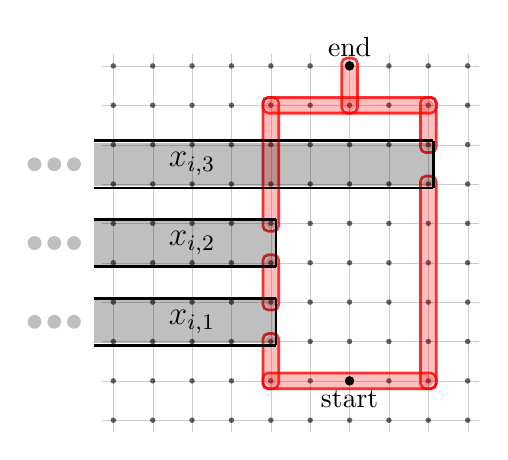
\begin{tikzpicture}[scale=0.50]
\def\wi{0.08}
\def\op{0.2}
\def\pts{2.0pt}
\foreach \x in {-6,...,3} {
\foreach \y in {-1,...,8} {
\fill[black, opacity=0.6] (\x, \y) circle (\pts);
}
}

\foreach \x in {-6,...,3} {
\draw[black, line width = \wi, opacity=\op] (\x, -1.3) -- (\x, 8.3);
}
\foreach \y in {-1,...,8} {
    \draw[black, line width = \wi, opacity=\op] (-6.3,  \y) -- (3.3, \y);

}
%\draw[red, line width = 2.267716536pt]   (-2, 0) -- (2, 0);
\draw[red, line width=1pt, opacity=0.8, rounded corners=2pt] (-2.2, -0.2) rectangle (2.2, 0.2);
\fill[red, opacity=0.25, rounded corners=5pt] (-2.2, -0.2) rectangle (2.2, 0.2);

%\draw[red, line width = 2.267716536pt]   (-2, 0) -- (-2, 1);

\draw[red, line width=1pt, opacity=0.8, rounded corners=2pt] (-2.2, -0.2) rectangle (-1.8, 1.2);
\fill[red, opacity=0.25, rounded corners=5pt] (-2.2, -0.2) rectangle (-1.8, 1.2);

% \draw[red, line width = 2.267716536pt]   (-2, 2) -- (-2, 3);

\draw[red, line width=1pt, opacity=0.8, rounded corners=2pt] (-2.2, 1.8) rectangle (-1.8, 3.2);
\fill[red, opacity=0.25, rounded corners=5pt] (-2.2, 1.8) rectangle (-1.8, 3.2);

% \draw[red, line width = 2.267716536pt]   (-2, 4) -- (-2, 7);


\draw[red, line width=1pt, opacity=0.8, rounded corners=2pt] (-2.2, 3.8) rectangle (-1.8, 7.2);
\fill[red, opacity=0.25, rounded corners=5pt] (-2.2, 3.8) rectangle (-1.8, 7.2);


% \draw[red, line width = 2.267716536pt]   (2, 0) -- (2, 5);


\draw[red, line width=1pt, opacity=0.8, rounded corners=2pt] (1.8, -0.2) rectangle (2.2, 5.2);
\fill[red, opacity=0.25, rounded corners=5pt] (1.8, -0.2) rectangle (2.2, 5.2);

%\draw[red, line width = 2.267716536pt]   (2, 6) -- (2, 7);


\draw[red, line width=1pt, opacity=0.8, rounded corners=2pt] (1.8, 5.8) rectangle (2.2, 7.2);
\fill[red, opacity=0.25, rounded corners=5pt] (1.8, 5.8) rectangle (2.2, 7.2);


%\draw[red, line width = 2.267716536pt]   (-2, 7) -- (2, 7);
\draw[red, line width=1pt, opacity=0.8, rounded corners=2pt] (-2.2, 6.8) rectangle (2.2, 7.2);
\fill[red, opacity=0.25, rounded corners=5pt] (-2.2, 6.8) rectangle (2.2, 7.2);

%\draw[red, line width = 2.267716536pt]   (0, 7) -- (0, 8);
\draw[red, line width=1pt, opacity=0.8, rounded corners=2pt] (-0.2, 6.8) rectangle (0.2, 8.2);
\fill[red, opacity=0.25, rounded corners=5pt] (-0.2, 6.8) rectangle (0.2, 8.2);

\filldraw (0, 0) circle (3pt);
\node[below] at (0, 0) {start};
\filldraw (0, 8) circle (3pt);
\node[above] at (0, 8) {end};
%\draw[red, line width=1pt, opacity=0.8, rounded corners=2pt] (-0.2, 6.8) rectangle (0.2, 8.2);
\draw[black, line width = 1pt]   (-6.5, 2.1) -- (-1.87, 2.1);
\draw[black, line width = 1pt]   (-6.5, 0.9) -- (-1.87, 0.9);
\draw[black, line width = 1pt]   (-1.87, 2.1) -- (-1.87, 0.9);
\draw[black, line width = 1pt]   (-6.5, 4.1) -- (-1.87, 4.1);
\draw[black, line width = 1pt]   (-6.5, 2.9) -- (-1.87, 2.9);
\draw[black, line width = 1pt]   (-1.87, 4.1) -- (-1.87, 2.9);
\draw[black, line width = 1pt]   (-6.5, 6.1) -- (2.13, 6.1);
\draw[black, line width = 1pt]   (-6.5, 4.9) -- (2.13, 4.9);
\draw[black, line width = 1pt]   (2.13, 6.1) -- (2.13, 4.9);
\draw[black, opacity=0.25, line width = 15.590551185000002pt]   (-6.5, 1.5) -- (-1.87, 1.5);
\draw[black, opacity=0.25, line width = 15.590551185000002pt]   (-6.5, 3.5) -- (-1.87, 3.5);
\draw[black, opacity=0.25, line width = 15.590551185000002pt]   (-6.5, 5.5) -- (2.13, 5.5);
\fill[black, opacity=0.25] (-7, 1.5) circle (5pt);
\fill[black, opacity=0.25] (-7.5, 1.5) circle (5pt);
\fill[black, opacity=0.25] (-8, 1.5) circle (5pt);
\node at (-4, 1.5) { \large $x_{i, 1}$};
\fill[black, opacity=0.25] (-7, 3.5) circle (5pt);
\fill[black, opacity=0.25] (-7.5, 3.5) circle (5pt);
\fill[black, opacity=0.25] (-8, 3.5) circle (5pt);
\node at (-4, 3.5) { \large $x_{i, 2}$};
\fill[black, opacity=0.25] (-7, 5.5) circle (5pt);
\fill[black, opacity=0.25] (-7.5, 5.5) circle (5pt);
\fill[black, opacity=0.25] (-8, 5.5) circle (5pt);
\node at (-4, 5.5) { \large $x_{i, 3}$};
\end{tikzpicture}
%[Finished in 0.2s]
    \caption{Depiction of the variable gadget of $x_i$. It consists of 8 fast agents (red). To deliver the package from ``start'' to ``end'', it must traverse either the left or right side of the gadget. For the left side, both $x_{i, 1}$ and $x_{i, 2}$ must be present to deliver the package across the two gaps; while for the right side, only $x_{i, 3}$ is required to cover a single gap. 
    Note that skipping the gadget and traversing the distance $a$ horizontally using a literal agent is too slow and therefore not feasible for satisfiable inputs.}
    %Note that skipping the gadget and traversing distance $a$ horizontally via some literal agent is too slow and will not be feasible for satisfiable inputs.}}
    \label{fig:grid_var_gadget}
\end{figure}

% \begin{figure}[h!]
%     \centering
%     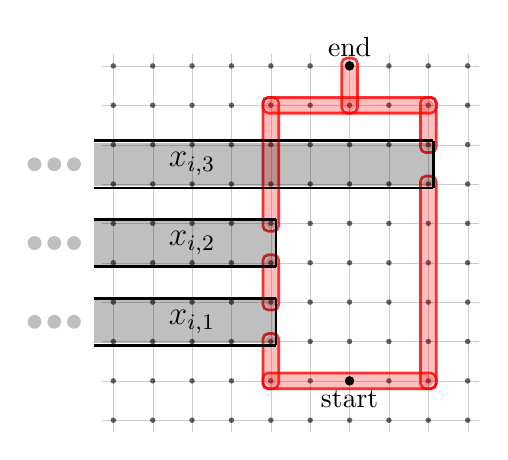
\begin{tikzpicture}[scale=0.50]
\def\wi{0.08}
\def\op{0.2}
\def\pts{2.0pt}
\foreach \x in {-6,...,3} {
\foreach \y in {-1,...,8} {
\fill[black, opacity=0.6] (\x, \y) circle (\pts);
}
}

\foreach \x in {-6,...,3} {
\draw[black, line width = \wi, opacity=\op] (\x, -1.3) -- (\x, 8.3);
}
\foreach \y in {-1,...,8} {
    \draw[black, line width = \wi, opacity=\op] (-6.3,  \y) -- (3.3, \y);

}
%\draw[red, line width = 2.267716536pt]   (-2, 0) -- (2, 0);
\draw[red, line width=1pt, opacity=0.8, rounded corners=2pt] (-2.2, -0.2) rectangle (2.2, 0.2);
\fill[red, opacity=0.25, rounded corners=5pt] (-2.2, -0.2) rectangle (2.2, 0.2);

%\draw[red, line width = 2.267716536pt]   (-2, 0) -- (-2, 1);

\draw[red, line width=1pt, opacity=0.8, rounded corners=2pt] (-2.2, -0.2) rectangle (-1.8, 1.2);
\fill[red, opacity=0.25, rounded corners=5pt] (-2.2, -0.2) rectangle (-1.8, 1.2);

% \draw[red, line width = 2.267716536pt]   (-2, 2) -- (-2, 3);

\draw[red, line width=1pt, opacity=0.8, rounded corners=2pt] (-2.2, 1.8) rectangle (-1.8, 3.2);
\fill[red, opacity=0.25, rounded corners=5pt] (-2.2, 1.8) rectangle (-1.8, 3.2);

% \draw[red, line width = 2.267716536pt]   (-2, 4) -- (-2, 7);


\draw[red, line width=1pt, opacity=0.8, rounded corners=2pt] (-2.2, 3.8) rectangle (-1.8, 7.2);
\fill[red, opacity=0.25, rounded corners=5pt] (-2.2, 3.8) rectangle (-1.8, 7.2);


% \draw[red, line width = 2.267716536pt]   (2, 0) -- (2, 5);


\draw[red, line width=1pt, opacity=0.8, rounded corners=2pt] (1.8, -0.2) rectangle (2.2, 5.2);
\fill[red, opacity=0.25, rounded corners=5pt] (1.8, -0.2) rectangle (2.2, 5.2);

%\draw[red, line width = 2.267716536pt]   (2, 6) -- (2, 7);


\draw[red, line width=1pt, opacity=0.8, rounded corners=2pt] (1.8, 5.8) rectangle (2.2, 7.2);
\fill[red, opacity=0.25, rounded corners=5pt] (1.8, 5.8) rectangle (2.2, 7.2);


%\draw[red, line width = 2.267716536pt]   (-2, 7) -- (2, 7);
\draw[red, line width=1pt, opacity=0.8, rounded corners=2pt] (-2.2, 6.8) rectangle (2.2, 7.2);
\fill[red, opacity=0.25, rounded corners=5pt] (-2.2, 6.8) rectangle (2.2, 7.2);

%\draw[red, line width = 2.267716536pt]   (0, 7) -- (0, 8);
\draw[red, line width=1pt, opacity=0.8, rounded corners=2pt] (-0.2, 6.8) rectangle (0.2, 8.2);
\fill[red, opacity=0.25, rounded corners=5pt] (-0.2, 6.8) rectangle (0.2, 8.2);

\filldraw (0, 0) circle (3pt);
\node[below] at (0, 0) {start};
\filldraw (0, 8) circle (3pt);
\node[above] at (0, 8) {end};
%\draw[red, line width=1pt, opacity=0.8, rounded corners=2pt] (-0.2, 6.8) rectangle (0.2, 8.2);
\draw[black, line width = 1pt]   (-6.5, 2.1) -- (-1.87, 2.1);
\draw[black, line width = 1pt]   (-6.5, 0.9) -- (-1.87, 0.9);
\draw[black, line width = 1pt]   (-1.87, 2.1) -- (-1.87, 0.9);
\draw[black, line width = 1pt]   (-6.5, 4.1) -- (-1.87, 4.1);
\draw[black, line width = 1pt]   (-6.5, 2.9) -- (-1.87, 2.9);
\draw[black, line width = 1pt]   (-1.87, 4.1) -- (-1.87, 2.9);
\draw[black, line width = 1pt]   (-6.5, 6.1) -- (2.13, 6.1);
\draw[black, line width = 1pt]   (-6.5, 4.9) -- (2.13, 4.9);
\draw[black, line width = 1pt]   (2.13, 6.1) -- (2.13, 4.9);
\draw[black, opacity=0.25, line width = 15.590551185000002pt]   (-6.5, 1.5) -- (-1.87, 1.5);
\draw[black, opacity=0.25, line width = 15.590551185000002pt]   (-6.5, 3.5) -- (-1.87, 3.5);
\draw[black, opacity=0.25, line width = 15.590551185000002pt]   (-6.5, 5.5) -- (2.13, 5.5);
\fill[black, opacity=0.25] (-7, 1.5) circle (5pt);
\fill[black, opacity=0.25] (-7.5, 1.5) circle (5pt);
\fill[black, opacity=0.25] (-8, 1.5) circle (5pt);
\node at (-4, 1.5) { \large $x_{i, 1}$};
\fill[black, opacity=0.25] (-7, 3.5) circle (5pt);
\fill[black, opacity=0.25] (-7.5, 3.5) circle (5pt);
\fill[black, opacity=0.25] (-8, 3.5) circle (5pt);
\node at (-4, 3.5) { \large $x_{i, 2}$};
\fill[black, opacity=0.25] (-7, 5.5) circle (5pt);
\fill[black, opacity=0.25] (-7.5, 5.5) circle (5pt);
\fill[black, opacity=0.25] (-8, 5.5) circle (5pt);
\node at (-4, 5.5) { \large $x_{i, 3}$};
\end{tikzpicture}
%[Finished in 0.2s]
%     \caption{\andi{Depiction of the variable gadget of $x_i$: The package has to traverse either the left or the right side of the gadget. For the left side, both $x_{i, 1}$ and $x_{i, 2}$ must present to deliver the package over the two gaps while for the right side, only $x_{i, 3}$ must be present to cover one gap. Note that skipping the gadget and traversing distance $a$ horizontally via some literal agent is too slow and will not be feasible for satisfiable inputs.}}
%     \label{fig:grid_var_gadget}
% \end{figure}
%old end of the caption
% In this example, clause $c_1$ includes the literals $x_1$, $\neg x_2$, and $x_3$; clause $c_2$ contains $x_1$ and $\neg x_n$; clause $c_{m'-1}$ consists of $\neg x_1$ and $x_{n'}$; and clause $c_m'$ contains $x_{n'}$ On the right side all the variable gadgets are stacked vertically. On the left side all the clause agents can move on parallel lines with a vertical gap of $a$.
 
 We now state the DDT-GridR instance formally and provide a proof of Theorem \ref{thm:grid_2speed}.

\paragraph*{Proof of Theorem 2.}
\label{sec:appendixddtgrapx}

%\thmgrid*

%Let $t$ be the size of the grid, i.e. the number of vertices. 
Let $\phi$ be the input formula of \textsc{2P1N-SAT} with $n'$ variables and $m'$ clauses. Observe that $m' \leq 3n'$.  %. and $n=a\cdot 8n'(m'+1)$. 
% \begin{theorem}
%     DDTGR is $n^{1-\varepsilon}$-APX-hard.
% \end{theorem}
We will now formally state the DDT-GridR instance $I$, describing each agent by its speed and movement area. The speed of the fast agents is set to $a-1$ and the slow agent speed to $1$. We set the starting point of the package to be $s = (0,0)$ and the destination to be $y = (-(m'+1)\cdot a,8n')$ where $n'$ is the number of variables and $m'$ is the number of clauses in the \textsc{2P1N-3SAT} instance $\phi$ and $a$ is a large integer that is set in the proof, depending on $n'$ and $\varepsilon$. Note that $a$ is also the horizontal spacing between clause gadgets as well as the transition from variable to clause gadgets.

Notice that each variable gadget $i$ consist of $8$ fast agents see Fig \ref{fig:grid_var_gadget}) with the following rectangular movement areas: $\forall i \in \{1, \dots, n'\}: $ 
\begin{itemize}
    \item[$\bullet$] $(a-1, [-2, 2] \times [8\cdot(i-1), 8\cdot(i-1)])$
    \item[$\bullet$] $ (a-1, [-2, -2] \times [8\cdot(i-1), 8\cdot(i-1)+1])$
    \item[$\bullet$] $(a-1, [-2,-2] \times [ 8\cdot(i-1)+2, 8\cdot(i-1)+3])$ 
    \item[$\bullet$] $(a-1, [-2, -2] \times [8\cdot(i-1)+4, 8\cdot(i-1)+7])$ 
    \item[$\bullet$] $(a-1, [2, 2] \times [8\cdot(i-1), 8\cdot(i-1)+5])$
    \item[$\bullet$] $(a-1, [2, 2] \times [8\cdot(i-1)+6, 8\cdot(i-1)+7])$
    \item[$\bullet$] $(a-1, [-2, 2] \times [8\cdot(i-1)+7, 8\cdot(i-1)+7])$
    \item[$\bullet$] $(a-1, [0, 0] \times [8\cdot(i-1)+7, 8\cdot(i-1)+8])$
\end{itemize}
Recall that since we are in the setting of no initial positioning, the agents are triples as the initial position $p_a$ is not specified in the instance.

As defined, $x_{i, 1}$ and $x_{i, 2}$ represent the positive literals of $x_i$, and $x_{i, 3}$ the negative literal. For each literal $x_{i, k}$, we denote $c_{j_{i, k}}$ as the clause that includes the literal $x_{i, k}$. The remaining agents are identified by their respective names.

\begin{itemize}
\item 
Each clause gadget $j$ consist of a fast agents with the following rectangular movement area:  $\forall j \in \{1, \dots, m'\}: $ 

\begin{itemize}
    \item[$\bullet$] agent $c_j$:  $(a-1, [-j\cdot a, -j\cdot a] \times [0, 8n'])$
\end{itemize}
\item Additionally there is an auxiliary agent $c_h$: $(a-1, [-(m'+1)\cdot a, -(m'+1)\cdot a] \times [0, 8n'])$

\item  %\andi{I would rather call this: The literal agents $x_{i,1},x_{i, 2}, x_{i, 3}$ and their respective counterparts $x'_{i,1},x'_{i, 2}, x'_{i, 3}$ ... depicted in Figure \ref{fig:grid_2speed} as grey bars}
For each variable $x_i$ we introduce the $3$ slow literal agents $x_{i, 1}, x_{i, 2}, x_{i, 3}$ and their respective counterparts $x'_{i,1},x'_{i, 2}, x'_{i, 3}$, depicted as gray bars and red lines, respectively in Figure \ref{fig:grid_2speed}. Formally they are defined using their speeds and movement areas:  
$\forall i \in \{1, \dots, n'\}: $ 
\begin{itemize}
    \item[$\bullet$] agent $ x_{i, 1}$:  $(1, [-j_{i, 1}\cdot a-1, -2] \times [8(i-1) + 1, 8(i-1) + 2])$
   \item[$\bullet$] agent $ x_{i, 2} $:  $ (1, [-j_{i, 2}\cdot a-1, -2]  \times [8(i-1) + 3, 8(i-1) + 4] )$
\item[$\bullet$] agent $ x_{i, 3} $:  $  (1, [-j_{i, 3}\cdot a-1, 2] \times [8(i-1) + 5, 8(i-1) + 6] )$
   \item[$\bullet$] agent $ x_{i, 1}'  $:  $ (a-1, [-(j_{i, 1}+1)\cdot a, -j_{i, 1}\cdot a-1]  \times [8(i-1) + 1, 8(i-1) + 1])$
  \item[$\bullet$] agent $ x_{i, 2}' $:  $ (a-1, [-(j_{i, 2}+1)\cdot a, -j_{i, 2}\cdot a-1] \times [8(i-1) + 3, 8(i-1) + 3]) $
 \item[$\bullet$] agent $ x_{i, 3}' $:  $(a-1, [-(j_{i, 3}+1)\cdot a, -j_{i, 3}\cdot a-1]  \times [8(i-1) + 5, 8(i-1) + 5]) $
\end{itemize}

\item In addition, we have a fast auxiliary agent $g$ dedicated to deliver the package from last variable gadget to the first clause gadget defined as: 
\begin{itemize}
    \item[$\bullet$] $ g:  (a-1, [-a, 0] \times [8n', 8n'])$,
\end{itemize}
\end{itemize}
Therefore, we have for the size of the grid $n$ that $n\leq 8n'(a\cdot (m'+1)+3)$.
We set the threshold value $t$ to be $n'^3$, i.e. in order to show $n^{1-\varepsilon}$-APX-hardness, we need to show that for any $n^{1-\varepsilon}$-approximation algorithm $A$ it holds, that $\phi$ is satisfiable if and only if the delivery time $t_A(I) \leq n^{1-\varepsilon}(n')^3$, where we define $a:=\left\lceil (n')^{\frac{6}{\varepsilon}} \right\rceil+1$.
%$ > \frac{(8(n')^4(m'+1))^{1/\varepsilon}}{8(m'+1)n'}$.\\

\begin{enumerate}
\item[$\implies$:]
$\phi$ is satisfiable, so let $\mathbf{x}$ be a satisfying assignment.\\
Given a variable $x_i$, we refer to the clauses that contain $x_{i, 1}$, $x_{i, 2}$ and $x_{i, 3}$ as $c_{j_1}$, $c_{j_2}$ and  $c_{j_3}$, respectively.

If $\mathbf{x}_i = 0$, we set the positions of both slow agents corresponding to the positive literals $x_{i,1}$ and $x_{i,2}$ to be at the variable gadget of $x_i$, i.e., at $(-2, 8(i-1) + 1)$ and $(-2, 8(i-1) + 3)$, respectively. The position of the slow agent corresponding to the negative literal $x_{i,3}$ is set to be on the vertical line of $c_{j_3}$, i.e., at $(-j_3\cdot a, 8(i-1) + 5)$, which is one unit before the start of $x_{i,3}'$.

If $\mathbf{x}_i = 1$, the position of $x_{i,3}$ is set to be at the variable gadget of $x_i$, i.e., at $(2, 8(i-1) + 5)$. The position of $x_{i,1}$ is set to be on the vertical line of $c_{j_1}$, at $(-j_1\cdot a, 8(i-1) + 1)$, one unit to the right of $x_{i,1}'$ and $x_{i,2}$ is set to be on the line of $c_{j_2}$, so at $(-j_2\cdot a, 8(i-1) + 3)$, one unit to the right of $x_{i,2}'$. 

Thus, for each variable $x_i$, either $x_{i,1}$ and $x_{i,2}$ are positioned at the variable gadget, or $x_{i,3}$ is positioned there. This configuration allows each gadget to be traversed in at most $12$ time units and point $B$ can be reached in time $12n'$. Next, $c_1$ is reached after an additional $\frac{a}{a-1}\leq 2$ time units with auxiliary agent $g$.

Let $x_{i,k}$ be a true literal of $c_1$ in the fulfilling assignment $\mathbf{x}$. We travel with agent $c_1$ to $(-a, 8(i-1) + 2k - 1)$ to the meeting point with $x_{i,k}$ (in at most $8n'$ time steps), and then one unit to the left with $x_{i,k}$ (in one time step) to bridge the gap and reach the movement area of $x_{i,k}'$. The agent $x_{i,k}$ is present at $c_1$, since either $k \in \{1, 2\}$ with $\mathbf{x}_i = 1$, setting $x_{i,k}$ at $c_1$, or $k = 3$ with $\mathbf{x}_i = 0$, also setting $x_{i,k}$ at $c_1$. Then, $x_{i,k}$ is used to reach $c_2$ in $\frac{a-1}{a-1}=1$ time step. This process is repeated for all other clause drones $c_3, \dots, c_m'$, each taking time $2+8n'$. Finally, $y$ is reached by $c_h$, which can be done in $8n'$ time. 
Thus, travelling from
\begin{itemize}
    \item from $s$ to $B$ takes time at most $12n'$
    \item from $B$ to $c_1$ takes time $\leq 2$
    \item from $c_1$ to $c_h$ takes time at most $m' (2+8n')$
    \item from $c_{m'}$ to $y$ takes time at most $8n'$
\end{itemize}
Therefore the total time of the optimal schedule is at most $12n'+2+m'\cdot(2+8n')+8n'$, which is $\leq n'^3$ for sufficiently large instances, therefore $t_A(I) \leq n^{1-\varepsilon}n'^3$.

\item[$\impliedby$:] 
Let $S$ be the schedule returned by algorithm $A$ with duration $t_A(I) \leq n^{1-\varepsilon}\cdot n'^3$. We observe that for sufficiently large instances the grid has size $n=8n'(a\cdot(m'+1)+3) \leq 16n'm'\cdot a \leq n'^3\cdot a$, therefore we can infer
\begin{equation}\label{eq}
    a < n < n'^3\cdot a
\end{equation}
We now show that in $S$, no literal agent can deliver the package over a horizontal distance of $a-1$ or more. 
Suppose there is a literal agent with speed 1 that covers a distance of $a-1$ or more. Then in total, 
$$
\begin{alignedat}{3}
    t_A(I)& > a  && > n'^{\frac{6}{\varepsilon}} \\
    &\iff  a^{\varepsilon} &&> n'^6 \\
    &\stackrel{\mathclap{(\ref{eq})}}{\implies} n^{\varepsilon} &&> n'^6 \\
    &\iff  \frac{1}{n'^6} &&> n^{-\varepsilon} \\
    &\iff  \frac{n}{n'^6} &&> n^{1-\varepsilon} \\
    &\stackrel{\mathclap{(\ref{eq})}}{\implies}  \frac{n'^3 \cdot a}{n'^6} &&> n^{1-\varepsilon} \\
    &\iff  a &&> n^{1-\varepsilon}\cdot n'^3 
\end{alignedat}
$$
therefore $t_A(I) > n^{1-\varepsilon}\cdot n'^3$, which contradicts the bound.
%\andi{all t's should be n's right`? please check yes, thanks}
%$w_A(I) > a > (8n^4m(8mn)^{-\varepsilon})^{1/\varepsilon}$ \\
%$ / OPT > t^{1-\varepsilon}$

% The difference between the $x$-coordinates of $A$ and $y$ is $n^3(m + 1)$. If a slow drone was to cover $n^3$ of this distance, the total delivery would require at least $n^5+n^3 + \frac{1}{2} \cdot n^3\cdot m = n^5+(m+2)(\frac{1}{2}\cdot n^3)$ time, which contradicts the bound, because $$n^5+(m+2)(\frac{1}{2} \cdot n^3) \leq n^5+\frac{1}{2} \cdot n^3(m + 1) + 13n(m + 2)$$
% $$\iff \frac{1}{2} \cdot n^3 \leq 13n(m + 2) \leq 28n^2$$
% which is false for sufficiently large $n$. Note that because $\phi$ is a 2P1N-Instance, $m \leq 2n$ holds.\\
Thus, a single slow literal agent cannot deliver the package directly from a variable gadget to $c_1$ or between clauses without violating our time constraint. Similarly, an agent cannot appear at two points separated by more than $a-1$ units.
Therefore, the package must pass through $B$ and utilize agent $g$, meaning for each variable gadget of $x_i$, either $x_{i,1}$ and $x_{i,2}$ are present for traversing the left path, or $x_{i,3}$ is present for the right path. In the former case, we set $x_i = 0$ (false), and in the latter, $x_i = 1$ (true). 
This construction yields a feasible assignment. It remains to show that this assignment is also satisfying.

To deliver the package to $y$, it must first reach $c_1$, then $c_2$, $c_3$ and subsequently $c_{m'}$ and $c_h$. Since taking the package from $c_{j}$ to $c_{j+1}$ requires a fast agent, we need an agent $x_{i, k}'$, such that $x_{i, k}$ is a literal in clause $c_j$. Then $x_{i, k}$ is needed to bridge the gap from $c_{j}$ to $x_{i,k}'$. 
If $k \in \{1, 2\}$ (indicating that $x_{i, k}$ is a positive literal), then $x_{i,3}$ must be present at the variable gadget. Thus, in our assignment, $x_i = 1$, so $c_{j}$ is satisfied. Conversely, if $k = 3$ (indicating $x_{i, k}$ is a negative literal), then $x_{i,1}$ and $x_{i,2}$ must be at the variable gadget, so $x_i = 0$, satisfying $c_j$. 

This observation translates to all clause gadgets as we derived that they are traversed without using a single literal agent for at least $a-1$ steps. Thus, all clauses are satisfied, making the assignment satisfying. Therefore, $\phi$ is satisfiable.

\end{enumerate}
This rounds up the proof of Theorem \ref{thm:grid_2speed}.\qed

Interestingly, the presented construction also has implications for the setting of initial positioning. %these results can be applied to the setting of initial positioning. 
The idea is to not start immediately at $s$ with the variable gadgets but start with a sufficiently large delay. If the delay is large enough, the literal agents can position themselves regardless of their initial starting point. However, note that this only establishes that the problem is NP-hard; it does not prove that the problem cannot be approximated within $O(n^{1-\varepsilon})$. We lose the inapproximability result due to the inclusion of a significant delay as part of every solution. Additionally, it is worth noting that the results from Theorem \ref{thm:line} do not directly apply to our setting on the unit grid with initial positions. The issue arises because, on a unit grid, for potentially exponentially large input values (with respect to the size of the encoding of the input), we would require $\Omega(P)$ vertices, where 
$P$ is the sum of all elements in the Partition input.

%      % First, we will consider cases with initial positioning. Later, we will modify the construction to obtain the same result for cases without initial positioning.

%     For a given input $\phi$ for \textsc{2P1N-3SAT} \simon{with $n'$ variables and $m'$ clauses}, we construct an instance for DDTGR as shown in Figure~\ref{fig:grid_2speed}. 
%     Let us first consider the variable gadget for each $x_i$ depicted in Figure \ref{fig:grid_var_gadget}.  For every variable $x_i$, we create three slow agents: two represent the positive  occurrences ($x_{i,1},x_{i,2}$) and one represents the negative occurrence ($x_{i,3}$). The high level idea is that the agents have to make a choice to either help with solving the clause gadgets on the left side or help getting through the variable gadget on the right side. 


 



%     We want to traverse from the bottom to the top using multiple fast agents (each depicted by a straight red line). To achieve this, the package must be transported across either both holes on the left or the single hole on the right.
%     %We want to get from bottom to top using multiple fast agents (every straight red line). Achieving this requires to have the package carried over either both holes on the left or the single hole on the right.
%     Three slow agents,  $x_{i,1}$ and $x_{i,2}$ for the positive occurrence on the left side, and $x_{i,3}$  for the negative occurrence on the right side, are designated to deliver the package over these three holes.  
%   Either the negative variable or both positive variables must engage with the variable gadget. By incorporating a variable gadget for  for every $x_i$ in $\phi$, we intuitively enforce a feasible assignment. Any unused  variable agents are available to help in traversing the clause gadgets on the opposite side. In addition to creating a variable gadget for each variable $x_i$, we also create three additional agents for each,  $x'_{i, 1}$,  $x'_{i, 2}$ and $x'_{i, 3}$, prepared to connect with the clause agents on the left side. 

%   A clause gadget is straightforward. For a clause $c_j$, we have one fast agent ($c_j$) which is able to traverse the entire grid vertically, and up to three fast agents corresponding to each respective literal ($x'$ agents). A clause is fulfilled whenever at least one literal is set to true. Therefore, we require one variable agent that corresponds to one of the literals to carry the package over the gap, delivering it to the respective $x'$ agent. Note that this variable agent can not help with its own variable gadget as the agent is slow and the horizontal distance is too large. \simon{We denote the horizontal distance between the clauses as $a$ and will set the ratio of the speeds of the fast and the slow agents to $a-1$. In the more technical part of the proof we will then choose a value for $a$ that depends on $\varepsilon$ and is so large, it ensures that travelling this horizontal distance with a slow agent takes more than $n^{1-\varepsilon}$ times the optimal delivery time for a satisfiable 2P1N-SAT instance $I$.} According to the \textsc{2P1N-3SAT} problem, we know that every variable has two positive and one negative occurrence, ensuring it's impossible that more than two positive variable agents ($x_{i,1},x_{i,2}$) or the one negative variable agent ($x_{i,3}$) are needed.\\



%     If there exists a feasible assignment for $\phi$, then an assignment exists for the variable agents to carry the package through the variable gadget and all clause gadgets, without requiring any variable agent to bridge more than a single gap. Once we have a variable agent cover more than one gap, achieving the optimal schedule becomes unfeasible.% Additionally, it is important to mention that we require a \emph{delay} agent $d$, as in Section \ref{npline}, to ensure every variable agent has sufficient time in its empty phase to reach its designated helping spot (variable gadget's hole or clause gadget's gap).

% Due to page limitations, the formal DDTGR instance is provided in the Appendix~\ref{sec:appendixddtgrapx}.

% It is important to note that this proof is also applicable to settings without initial positions:  In this case, from a setting with initial positions to one without requires not much effort. Notably, the delay agent $d$ is no longer necessary, as every variable agent can be precisely positioned to carry the package over some gap. It is still essential to traverse the variable gadget from bottom to top, ensuring feasible assignments.
%     \qed

% Note that the reason this transformation works here but not in the construction in Section \ref{npline} is that we do not depend on precise timing in our grid construction. However, on the line, we depended on meeting the delay agent $p$ at exactly the right moment, and it is not feasible to establish holes or gaps on a line since the package's delivery path is fixed and unique. In a setting without initial positions, agent $p$ might just be placed on the left and the entire construction is ineffective. 

%Prior work by Erlebach et al.~\cite{erlebach:drones} demonstrates that the problem with a single speed can be solved in polynomial time. Our results extend this understanding by addressing the case of two speeds on a unit grid graph in both with and without initial positions. 

%\subsubsection{An easy tight approximation algorithm}
\subsection*{A simple $O(n)$-approximation for DDT-GridR on a unit grid}
We now demonstrate that, in the setting of %unweighted graphs—a generalization of 
unit grid graphs with different speeds a simple greedy algorithm achieves an \( n \)-approximation. Notably, this result is near-optimal due to Theorem \ref{thm:grid_2speed}, as no $O(n^{1-\varepsilon})$-approximation algorithm for any $\varepsilon > 0$ exists, unless P$=$NP. 
%
% \begin{theorem}
%     There exists an \( O(n) \)-approximation algorithm for DDT on unweighted graphs.
% \end{theorem}
%

The proposed algorithm begins by sorting the agents in non-increasing order of speed and iteratively attempts to find an (s-y)-path in the graph induced by the movement areas of only the fastest available agents. 
If a path cannot be found using the fastest agent, the algorithm progressively incorporates slower agents until a valid path is identified. Once a valid path is determined, a corresponding schedule can be constructed using the respective agents. 
%The proposed algorithm operates by sorting the agents by their speeds in non-increasing order and iteratively attempting to construct a \andi{(s-y)-path rather or, as schedule is constructed later}schedule using only the fastest available agents.  If a feasible schedule cannot be found with the fastest agent, the algorithm progressively incorporates slower agents until a valid schedule is identified.
%\simon{The proposed algorithm operates by sorting the agents by their speeds in non-increasing order and iteratively attempting to find a ($s$-$y$)-path in the graph induced by the movement areas of only the fastest agents. If a path cannot be found using the fastest agent, the algorithm progressively incorporates slower agents until a valid path is identified. Using this path a valid schedule can be constructed using the respective agents. }
The algorithm is presented as follows:

\begin{algorithm}[H]
\caption{Greedy $O(n)$-approximation}
\label{alg:greedy}
\begin{algorithmic}[1]
%\INPUT Drones \( a_1, \dots, a_k \) with speeds \( v_1, \dots, v_k \), sorted in non-decreasing order of speed.
%\OUTPUT A feasible schedule \( S' \) or confirmation of infeasibility.
\STATE Let the agents $a_1, \dots, a_k$ be sorted in non-increasing order of their speeds. 
\FOR{\( i = 1 \) to \( k \)}
    \IF{there exists a path \( P \) from \( s \) to \( y \) in graph \( (V_1 \cup \dots \cup V_i, E_1 \cup \dots \cup E_i) \)}
        \STATE Construct a feasible schedule \( S \) by assigning an agent \( a \in \{a_1, \dots, a_i\} \) to each edge \( e \in P \) such that \( e \in E_a \).
        \STATE Transform \( S \) into schedule \( S^* \) such that each agent is used at most once.   %(as shown in Section \ref{preliminaries}) %(using Lemma ?? from \cite{erlebach}).
      %  \STATE Transform \( S' \) into schedule \( S^* \) such that each vertex is visited at most once in $S^*$   %(using Lemma ?? from \cite{erlebach}).
        \RETURN \( S^* \)
    \ENDIF
\ENDFOR
\RETURN No feasible schedule exists.
\end{algorithmic}
\end{algorithm}
\noindent

During the construction of schedule $S$ in step 4, it is possible for a single agent to be used for multiple disjoint segments of the trip. However, we can convert $S$ into a schedule $S^*$ that uses each agent at most once  without increasing the total delivery time. 
Specifically, for any agent $a$, consider the first and last edge assigned to $a$ in $S$, say $\{u, v\}$ and $\{u', v'\}$, respectively. If there exist edges between $\{u, v\}$ and $\{u', v'\}$ in the schedule $S$ that are assigned to other agents, the schedule can be adjusted to deliver the package from $v$ to $v'$, removing the rest of the schedule in between $\{u, v\}$ and $\{u', v'\}$.  This ensures that each agent is used at most once, and consequently, the package never has to wait for any agent to arrive. Additionally, the agent will deliver the package from $u$ to $v'$ with the minimum total length, as each agent is constrained to a rectangular movement area within the grid. Furthermore, the length of the found ($s$-$y$)-path traversed by $S^*$ is upper-bounded by $n$.

The algorithm runs for at most \( k \) iterations. Each iteration requires \( O(n) \)-time to search for the path $P$ using a depth-first search (DFS). To construct $S^*$, we perform a DFS for each agent $a$ to find a direct path in $(V_a,E_a)$ from the first edge to the last edge assigned to $a$, resulting in $O(n\cdot k)$.   As Step 4-5 are done only once, the total runtime complexity is $O(n \cdot k + k \log k)$, which also includes the time required for sorting the agents.

 


% Specifically, for any agent $a$, consider the first and last edge assigned to $a$ in $S$, say $\{u, v\}$ and $\{u', v'\}$, respectively. If there exist edges between $\{u, v\}$ and $\{u', v'\}$ in the \andi{path proceeded by }schedule $S$ that are assigned to other agents, the schedule can be adjusted to deliver the package from \todo{why are we not saying from $u$ to $v'$ immediately?}$v$ to $u'$, removing the rest of the schedule in between $\{u, v\}$ and $\{u', v'\}$. This ensures that each agent is used at most once and consequently the package never has to wait for any agent to arrive. However, this transformation may lead to vertices being visited multiple times. If a vertex $u$ is visited more than once, we can just completely skip all trips between the first arrival and the last departure of $u$ to achieve schedule $S^*$. This guarantees that in $S^*$, each vertex is visited at most once and each agent is used at most once. \andi{Moreover, the length of the found ($s$-$y$)-path traversed by $S^*$ is upper-bounded by $n$.}
% The algorithm runs for at most \( k \) iterations. Each iteration requires \( O(n) \)-time to search for the path $P$ using a depth-first search (DFS). To construct $S'$, we perform a DFS for each agent $a$ to find a direct path \andi{in $(V_a,E_a)$} from the first edge to the last edge assigned to $a$, resulting in $O(n\cdot k)$. Simplifying $S'$ into $S^*$ involves iterating through $S'$ once and removing edges, which therefore can be done in $O(n\cdot k)$ time.  As Step 4-6 are done only once, the total runtime complexity is $O(n \cdot k + k \log k)$, which also includes the time required for sorting the agents.

% \todo{A: Maybe I would like a little theorem here with a proof environment, what do you think? S: For everything or just the approximation guarantee? Only guarantee. Let Kelin decide!}

Suppose the algorithm terminates after $i'$ iterations.
%Let \( i' \) denote the value of \( i \) at which the algorithm terminates and returns a solution.
Note that no feasible schedule exists using only the agents \( a_1, \dots, a_{i'-1} \); otherwise, the algorithm would have terminated in an earlier iteration. Consequently, in any feasible schedule, at least one edge (of unit length) must be traversed by an agent with speed at most \( v_{i'} \). Thus, \( OPT \geq 1 / v_{i'} \), with $OPT$ denoting the delivery time of an optimal schedule. 

Since the initial positions of every agent can be chosen and every agent is used at most once, the package never has to wait for any drone to arrive. Therefore, the delivery time of schedule $S^*$ is solely determined by the time spent delivering the package along the corresponding route. The total distance traveled by the package is at most \( n-1 \), and each agent in \( S^* \) has a speed of at least \( v_{i'} \). Therefore, for the total delivery time of schedule $S^*$ we conclude
\[
t(S^*) \leq \frac{n}{v_{i'}}.
\]
Combining this with \( OPT \geq \frac{1}{v_{i'}} \), the approximation guarantee of the algorithm is
\[
\frac{t(S^*)}{OPT} \leq \frac{\frac{n}{v_{i'}}}{\frac{1}{v_{i'}}} = n.
\]


% \begin{figure}[h]
%     \centering
%     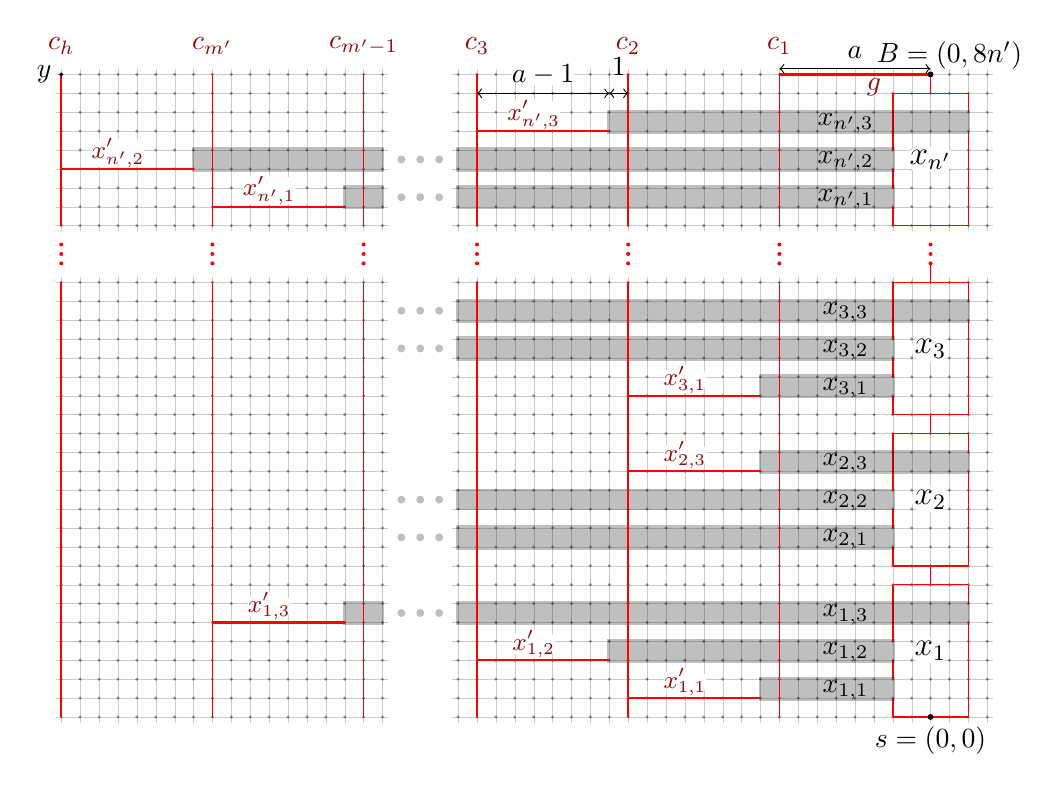
\begin{tikzpicture}[scale=0.24]
\definecolor{dred}{RGB}{143, 11, 11}
\def\wi{0.08}
\def\op{0.2}
\def\pts{2.5pt}

\foreach \x in {-25,...,3} {
\foreach \y in {0,...,23} {
\fill[black, opacity=0.4] (\x, \y) circle (\pts);
}
\draw[black, line width=\wi, opacity=\op] (\x, -0.3) -- (\x, 23.3);
}
\foreach \y in {0,...,23} {
\draw[black, line width=\wi, opacity=\op] (-25.3, \y) -- (3.3, \y);
\draw[black, line width=\wi, opacity=\op] (-46.3, \y) -- (-28.7, \y);
}
\foreach \y in {26,...,34} {
\draw[black, line width=\wi, opacity=\op] (-25.3, \y) -- (3.3, \y);
\draw[black, line width=\wi, opacity=\op] (-46.3, \y) -- (-28.7, \y);
}

\foreach \x in {-25,...,3} {
\foreach \y in {26,...,34} {
\fill[black, opacity=0.4] (\x, \y) circle (\pts);
}
\draw[black, line width=\wi, opacity=\op] (\x, 25.7) -- (\x, 34.3);
}


\foreach \x in {-46,...,-29} {
\foreach \y in {26,...,34} {
\fill[black, opacity=0.4] (\x, \y) circle (\pts);
}
\draw[black, line width=\wi, opacity=\op] (\x, 25.7) -- (\x, 34.3);

}
\foreach \x in {-46,...,-29} {
\foreach \y in {0,...,23} {
\fill[black, opacity=0.4] (\x, \y) circle (\pts);
}
\draw[black, line width=\wi, opacity=\op] (\x, -0.3) -- (\x, 23.3);
}
\draw[red, line width = 0.5669291340000001pt]   (-2, 0) -- (2, 0);
\draw[red, line width = 0.5669291340000001pt]   (-2, 0) -- (-2, 1);
\draw[red, line width = 0.5669291340000001pt]   (-2, 2) -- (-2, 3);
\draw[red, line width = 0.5669291340000001pt]   (-2, 4) -- (-2, 7);
\draw[red, line width = 0.5669291340000001pt]   (2, 0) -- (2, 5);
\draw[red, line width = 0.5669291340000001pt]   (2, 6) -- (2, 7);
\draw[red, line width = 0.5669291340000001pt]   (-2, 7) -- (2, 7);
\draw[red, line width = 0.5669291340000001pt]   (0, 7) -- (0, 8);
\node[fill=white, rounded corners, inner sep=1pt, outer sep=1pt] at (0, 3.5)  {\large $x_1$};
\draw[red, line width = 0.5669291340000001pt]   (-2, 8) -- (2, 8);
\draw[red, line width = 0.5669291340000001pt]   (-2, 8) -- (-2, 9);
\draw[red, line width = 0.5669291340000001pt]   (-2, 10) -- (-2, 11);
\draw[red, line width = 0.5669291340000001pt]   (-2, 12) -- (-2, 15);
\draw[red, line width = 0.5669291340000001pt]   (2, 8) -- (2, 13);
\draw[red, line width = 0.5669291340000001pt]   (2, 14) -- (2, 15);
\draw[red, line width = 0.5669291340000001pt]   (-2, 15) -- (2, 15);
\draw[red, line width = 0.5669291340000001pt]   (0, 15) -- (0, 16);
\node[fill=white, rounded corners, inner sep=1pt, outer sep=1pt] at (0, 11.5)  {\large $x_2$};
\draw[red, line width = 0.5669291340000001pt]   (-2, 16) -- (2, 16);
\draw[red, line width = 0.5669291340000001pt]   (-2, 16) -- (-2, 17);
\draw[red, line width = 0.5669291340000001pt]   (-2, 18) -- (-2, 19);
\draw[red, line width = 0.5669291340000001pt]   (-2, 20) -- (-2, 23);
\draw[red, line width = 0.5669291340000001pt]   (2, 16) -- (2, 21);
\draw[red, line width = 0.5669291340000001pt]   (2, 22) -- (2, 23);
\draw[red, line width = 0.5669291340000001pt]   (-2, 23) -- (2, 23);
\draw[red, line width = 0.5669291340000001pt]   (0, 23) -- (0, 24);
\node[fill=white, rounded corners, inner sep=1pt, outer sep=1pt] at (0, 19.5)  {\large$x_3$};
\draw[red, line width = 0.5669291340000001pt]   (-2, 26) -- (2, 26);
\draw[red, line width = 0.5669291340000001pt]   (-2, 26) -- (-2, 27);
\draw[red, line width = 0.5669291340000001pt]   (-2, 28) -- (-2, 29);
\draw[red, line width = 0.5669291340000001pt]   (-2, 30) -- (-2, 33);
\draw[red, line width = 0.5669291340000001pt]   (2, 26) -- (2, 31);
\draw[red, line width = 0.5669291340000001pt]   (2, 32) -- (2, 33);
\draw[red, line width = 0.5669291340000001pt]   (-2, 33) -- (2, 33);
\draw[red, line width = 0.5669291340000001pt]   (0, 33) -- (0, 34);
\node[fill=white, rounded corners, inner sep=1pt, outer sep=1pt] at (0, 29.5)  {\large $x_{n'}$};
\draw[black, line width = 8.736220474000001pt, opacity=0.25]   (-9.1, 1.5) -- (-1.9, 1.5);
\node at (-4.5, 1.4) { $x_{1, 1}$};
\draw[black, line width = 8.736220474000001pt, opacity=0.25]   (-17.1, 3.5) -- (-1.9, 3.5);
\node at (-4.5, 3.4) { $x_{1, 2}$};
\draw[black, line width = 8.736220474000001pt, opacity=0.25]   (-25.1, 5.5) -- (2.1, 5.5);
\node at (-4.5, 5.4) { $x_{1, 3}$};
\fill[black, opacity=0.25] (-26, 5.5) circle (6pt);
\fill[black, opacity=0.25] (-27, 5.5) circle (6pt);
\fill[black, opacity=0.25] (-28, 5.5) circle (6pt);
\draw[black, line width = 8.736220474000001pt, opacity=0.25]   (-31.1, 5.5) -- (-28.9, 5.5);
\draw[black, line width = 8.736220474000001pt, opacity=0.25]   (-25.1, 9.5) -- (-1.9, 9.5);
\node at (-4.5, 9.4) { $x_{2, 1}$};
\fill[black, opacity=0.25] (-26, 9.5) circle (6pt);
\fill[black, opacity=0.25] (-27, 9.5) circle (6pt);
\fill[black, opacity=0.25] (-28, 9.5) circle (6pt);
\draw[black, line width = 7.836220474000001pt, opacity=0.25]   (-25.1, 11.5) -- (-1.9, 11.5);
\node at (-4.5, 11.4) { $x_{2, 2}$};
\fill[black, opacity=0.25] (-26, 11.5) circle (6pt);
\fill[black, opacity=0.25] (-27, 11.5) circle (6pt);
\fill[black, opacity=0.25] (-28, 11.5) circle (6pt);
\draw[black, line width = 8.736220474000001pt, opacity=0.25]   (-9.1, 13.5) -- (2.1, 13.5);
\node at (-4.5, 13.4) { $x_{2, 3}$};
\draw[black, line width = 8.736220474000001pt, opacity=0.25]   (-9.1, 17.5) -- (-1.9, 17.5);
\node at (-4.5, 17.4) { $x_{3, 1}$};
\draw[black, line width = 8.736220474000001pt, opacity=0.25]   (-25.1, 19.5) -- (-1.9, 19.5);
\node at (-4.5, 19.4) { $x_{3, 2}$};
\fill[black, opacity=0.25] (-26, 19.5) circle (6pt);
\fill[black, opacity=0.25] (-27, 19.5) circle (6pt);
\fill[black, opacity=0.25] (-28, 19.5) circle (6pt);
\draw[black, line width = 8.736220474000001pt, opacity=0.25]   (-25.1, 21.5) -- (2.1, 21.5);
\node at (-4.5, 21.4) { $x_{3, 3}$};
\fill[black, opacity=0.25] (-26, 21.5) circle (6pt);
\fill[black, opacity=0.25] (-27, 21.5) circle (6pt);
\fill[black, opacity=0.25] (-28, 21.5) circle (6pt);
\draw[black, line width = 8.736220474000001pt, opacity=0.25]   (-25.1, 27.5) -- (-1.9, 27.5);
\node at (-4.5, 27.4) { $x_{n', 1}$};
\fill[black, opacity=0.25] (-26, 27.5) circle (6pt);
\fill[black, opacity=0.25] (-27, 27.5) circle (6pt);
\fill[black, opacity=0.25] (-28, 27.5) circle (6pt);
\draw[black, line width = 8.736220474000001pt, opacity=0.25]   (-25.1, 29.5) -- (-1.9, 29.5);
\node at (-4.5, 29.4) { $x_{n', 2}$};
\fill[black, opacity=0.25] (-26, 29.5) circle (6pt);
\fill[black, opacity=0.25] (-27, 29.5) circle (6pt);
\fill[black, opacity=0.25] (-28, 29.5) circle (6pt);
\draw[black, line width = 8.736220474000001pt, opacity=0.25]   (-17.1, 31.5) -- (2.1, 31.5);
\node at (-4.5, 31.4) { $x_{n', 3}$};
% \fill[black, opacity=0.25] (-26, 31.5) circle (6pt);
% \fill[black, opacity=0.25] (-27, 31.5) circle (6pt);
% \fill[black, opacity=0.25] (-28, 31.5) circle (6pt);
\draw[black, line width = 8.736220474000001pt, opacity=0.25]   (-31.1, 27.5) -- (-28.9, 27.5);
\draw[black, line width = 8.736220474000001pt, opacity=0.25]   (-39.1, 29.5) -- (-28.9, 29.5);
\node at (-8, 35.5)  {$\textcolor{dred}{c_1}$};
\draw[red, line width = 0.5669291340000001pt]   (-8, 0) -- (-8, 23);
\draw[red, line width = 0.5669291340000001pt]   (-8, 26) -- (-8, 34);
\fill[red] (-8, 24) circle (3pt);
\fill[red] (-8, 24.5) circle (3pt);
\fill[red] (-8, 25) circle (3pt);
\node at (-16, 35.5)  {$\textcolor{dred}{c_2}$};
\draw[red, line width = 0.5669291340000001pt]   (-16, 0) -- (-16, 23);
\draw[red, line width = 0.5669291340000001pt]   (-16, 26) -- (-16, 34);
\fill[red] (-16, 24) circle (3pt);
\fill[red] (-16, 24.5) circle (3pt);
\fill[red] (-16, 25) circle (3pt);
\node at (-24, 35.5)  {$\textcolor{dred}{c_3}$};
\draw[red, line width = 0.5669291340000001pt]   (-24, 0) -- (-24, 23);
\draw[red, line width = 0.5669291340000001pt]   (-24, 26) -- (-24, 34);
\fill[red] (-24, 24) circle (3pt);
\fill[red] (-24, 24.5) circle (3pt);
\fill[red] (-24, 25) circle (3pt);
\node at (-30, 35.5)  {$\textcolor{dred}{c_{m'-1}}$};
\draw[red, line width = 0.5669291340000001pt]   (-30, 0) -- (-30, 23);
\draw[red, line width = 0.5669291340000001pt]   (-30, 26) -- (-30, 34);
\fill[red] (-30, 24) circle (3pt);
\fill[red] (-30, 24.5) circle (3pt);
\fill[red] (-30, 25) circle (3pt);
\node at (-38, 35.5)  {$\textcolor{dred}{c_{m'}}$};
\draw[red, line width = 0.5669291340000001pt]   (-38, 0) -- (-38, 23);
\draw[red, line width = 0.5669291340000001pt]   (-38, 26) -- (-38, 34);
\fill[red] (-38, 24) circle (3pt);
\fill[red] (-38, 24.5) circle (3pt);
\fill[red] (-38, 25) circle (3pt);
\node at (-46, 35.5)  {$\textcolor{dred}{c_h}$};
\draw[red, line width = 0.5669291340000001pt]   (-46, 0) -- (-46, 23);
\draw[red, line width = 0.5669291340000001pt]   (-46, 26) -- (-46, 34);
\fill[red] (-46, 24) circle (3pt);
\fill[red] (-46, 24.5) circle (3pt);
\fill[red] (-46, 25) circle (3pt);
\fill[red] (0, 24) circle (3pt);
\fill[red] (0, 24.5) circle (3pt);
\fill[red] (0, 25) circle (3pt);
\draw[red, line width = 0.8503937010000002pt]   (-8, 34) -- (0, 34);
\draw[red, line width = 0.8503937010000002pt]   (-16, 1) -- (-9, 1);
\node[fill=white, rounded corners, inner sep=0pt, outer sep=0pt] at (-13, 1.85) { \small $\textcolor{dred}{x_{1, 1}'}$};
\draw[red, line width = 0.8503937010000002pt]   (-16, 13) -- (-9, 13);
\node[fill=white, rounded corners, inner sep=0pt, outer sep=0pt] at (-13, 13.85) { \small $\textcolor{dred}{x_{2, 3}'}$};
\draw[red, line width = 0.8503937010000002pt]   (-16, 17) -- (-9, 17);
\node[fill=white, rounded corners, inner sep=0pt, outer sep=0pt] at (-13, 17.85) { \small $\textcolor{dred}{x_{3, 1}'}$};
\draw[red, line width = 0.8503937010000002pt]   (-24, 3) -- (-17, 3);
\node[fill=white, rounded corners, inner sep=0pt, outer sep=0pt] at (-21, 3.85) { \small $\textcolor{dred}{x_{1, 2}'}$};
\draw[red, line width = 0.8503937010000002pt]   (-24, 31) -- (-17, 31);
\node[fill=white, rounded corners, inner sep=0pt, outer sep=0pt] at (-21, 31.85) { \small $\textcolor{dred}{x_{n', 3}'}$};
\draw[red, line width = 0.8503937010000002pt]   (-38, 5) -- (-31, 5);
\node[fill=white, rounded corners, inner sep=0pt, outer sep=0pt] at (-35, 5.85) { \small $\textcolor{dred}{x_{1, 3}'}$};
\draw[red, line width = 0.8503937010000002pt]   (-38, 27) -- (-31, 27);
\node[fill=white, rounded corners, inner sep=0pt, outer sep=0pt] at (-35, 27.85) { \small $\textcolor{dred}{x_{n', 1}'}$};
\draw[red, line width = 0.8503937010000002pt]   (-46, 29) -- (-39, 29);
\node[fill=white, rounded corners, inner sep=0pt, outer sep=0pt] at (-43, 29.85) { \small $\textcolor{dred}{x_{n', 2}'}$};
%\filldraw (0, -4) circle (2pt);
%\node[left] at (0, -4) {$s=(0, - n^5)$};
\filldraw (0, 0) circle (3.5pt);
\node[below] at (0, 0) {$s = (0, 0)$};
\filldraw (0, 34) circle (3.5pt);
\node[] at (1, 35) {$B = (0, 8n')$};
\filldraw (-46, 34) circle (2pt);
\node[left] at (-46, 34) {$y$};
\draw[<->] (-24, 33) -- (-17, 33) node[midway, above=3pt, fill=white, rounded corners, inner sep=0pt, outer sep=0pt] {$a-1$};
\draw[<->] (-17, 33) -- (-16, 33) node[midway, above=3pt] {$1$};
\draw[<->] (-8, 34.3) -- (0, 34.3) node[midway, above] {$a$};
%\draw[black, line width = 0.5669291340000001pt]   (0, 0) -- (0, -4);
%\node[left] at (0, -2)  {$d$};
\node[fill=white, rounded corners, inner sep=0pt, outer sep=0pt] at (-3, 33.3) {$\textcolor{dred}{g}$};
%\node[fill=white, rounded corners] at (0, 0) {$s$};
\end{tikzpicture}
%[Finished in 0.1s]
%     \caption{}
% \label{fig:grid_2speed}
% \end{figure}

%  Once we can get ride of the delay, in our hardness proof, e can present the following result regarding inapproximability:

% \begin{theorem}
%     For the setting without initial positions it is not possible to approximate DDTGR within any poly(n,k) approximation ratio.
% \end{theorem}
% \todo{review and move proof to Appendix}
% \begin{proof}
%     Observe that in the setting without initial positions an optimal schedule takes time $some-value$, assuming $\phi$ has a feasible assignment. If there does not exist a feasible assignment then a variable agent has to travel from right to left to fill a gap in the variable gadget and also fill a gap in some clause gadget(s). However travelling from right to left with a slow agent takes time $some-larger-value$. Therefore, if we could approximate DDTGR by a ratio of $-ratio-$, then we could solve \textsc{2P1N-3SAT}.
% \end{proof}


% \subsection{NP-Hardness for unit speed drones and arbitrary movement areas} 
% \label{1grid}
% We can adapt the core construction of section \ref{2grid} to achieve similar results for  agents with unit speed and arbitrary movement areas, though some adjustments are necessary. The construction in \ref{2grid} only works if the speed of the fast agents exceeds that of the slower (variable) agents. 
% Nevertheless, the flexibility of arbitrary movement areas allows us to cope with that.  Since we are not confined to rectangular paths, we can simulate slower speeds by requiring agents to take detours. The movement areas of the variable agents are depicted in Figure \ref{fig:grid_1speed}. By setting the vertical spacing of agents $x_{i,1},x_{i,2}$ and $x_{i,3}$ to 2, we can replicate the same speeds used in the construction for two speeds and rectangular movement areas. Therefore, the results are transferable, and we can state our result below. Due to space limitations, the proof is omitted. % We will not prove it but argue that the proof can be done analogously to the proof of Theorem \ref{thm:grid_2speed} in Appendix \ref{sec:appendixDDTGRproof}.

%\thmgridspeed* 

% \begin{proof}
%     We proof the theorem by arguing that there exist feasible values for $a$ and $b$ to model the case for the proof of Theorem \ref{thm:grid_2speed}. Note that the size of the grid does also not significantly grow. \todo{is that actually true, I dont know the values}
% \end{proof}


% \begin{theorem}
%     For the setting without initial positions it is not possible to approximate DDTG within any poly(n,k) approximation ratio.
% \end{theorem}
% \vspace{-2mm}
% \begin{figure}[h]
%     \centering
%     \input{grid_1speed}
%     \caption{A close up on a variable gadget (right side) as well as a clause gadget (left side)} for the DDTGU instance. The general construction does not differ from the DDTGR case. Due to the relaxation in movement areas, we make the variable agents $x_{i,1},x_{i,2},x_{i,3}$ move via large detours when traveling horizontally, somewhat introducing a second slow speed. Note that although we use different colors the agents' speeds are equal. 
% \label{fig:grid_1speed}
% \end{figure}


\section{Conclusion}
In this work, we propose a simple yet effective approach, called SMILE, for graph few-shot learning with fewer tasks. Specifically, we introduce a novel dual-level mixup strategy, including within-task and across-task mixup, for enriching the diversity of nodes within each task and the diversity of tasks. Also, we incorporate the degree-based prior information to learn expressive node embeddings. Theoretically, we prove that SMILE effectively enhances the model's generalization performance. Empirically, we conduct extensive experiments on multiple benchmarks and the results suggest that SMILE significantly outperforms other baselines, including both in-domain and cross-domain few-shot settings.


\bibliographystyle{splncs04}
\bibliography{refs}

\end{document}
